\section{PSE: Scalable Precise Entropy Computation}
\label{sec:PSE}

In this section, we introduce our computational tool, PSE, designed to calculate the Shannon entropy of a specified circuit CNF formula with respect to its output variables.
%Just like other Shannon entropy tools, the computing process of PSE is divided into two stages: $Y$-stage (corresponding to outputs) and $X$-stage (corresponding to inputs).
Similar to other Shannon entropy tools, the main process of PSE is divided into two stages: the $Y$-stage (corresponding to outputs) and the $X$-stage (corresponding to inputs).
In the $Y$-stage, we execute a targeted search within the ADD-L framework to accurately compute the Shannon entropy.%File: anonymous-submission-latex-2025.tex
\documentclass[letterpaper]{article} % DO NOT CHANGE THIS
\usepackage[submission]{aaai25}  % DO NOT CHANGE THIS
\usepackage{times}  % DO NOT CHANGE THIS
\usepackage{helvet}  % DO NOT CHANGE THIS
\usepackage{courier}  % DO NOT CHANGE THIS
\usepackage[hyphens]{url}  % DO NOT CHANGE THIS
\usepackage{graphicx} % DO NOT CHANGE THIS
\urlstyle{rm} % DO NOT CHANGE THIS
\def\UrlFont{\rm}  % DO NOT CHANGE THIS
\usepackage{natbib}  % DO NOT CHANGE THIS AND DO NOT ADD ANY OPTIONS TO IT
\usepackage{caption} % DO NOT CHANGE THIS AND DO NOT ADD ANY OPTIONS TO IT
\frenchspacing  % DO NOT CHANGE THIS
\setlength{\pdfpagewidth}{8.5in} % DO NOT CHANGE THIS
\setlength{\pdfpageheight}{11in} % DO NOT CHANGE THIS
%
% These are recommended to typeset algorithms but not required. See the subsubsection on algorithms. Remove them if you don't have algorithms in your paper.
%\usepackage{algorithm}
%\usepackage{algorithmic}


\usepackage{amsmath} 
\usepackage{amsthm}
\newtheorem{example}{Example}[section]
\newtheorem{proposition}{Proposition}[section]
\newtheorem{definition}{Definition}[section]
\usepackage[ruled,vlined]{algorithm2e}
\usepackage{comment}

\usepackage{graphicx}
\usepackage{booktabs}
\usepackage{multirow}


%
% These are are recommended to typeset listings but not required. See the subsubsection on listing. Remove this block if you don't have listings in your paper.
\usepackage{newfloat}
\usepackage{listings}
\DeclareCaptionStyle{ruled}{labelfont=normalfont,labelsep=colon,strut=off} % DO NOT CHANGE THIS
\lstset{%
	basicstyle={\footnotesize\ttfamily},% footnotesize acceptable for monospace
	numbers=left,numberstyle=\footnotesize,xleftmargin=2em,% show line numbers, remove this entire line if you don't want the numbers.
	aboveskip=0pt,belowskip=0pt,%
	showstringspaces=false,tabsize=2,breaklines=true}

%
% Keep the \pdfinfo as shown here. There's no need
% for you to add the /Title and /Author tags.
\pdfinfo{
	/TemplateVersion (2025.1)
}

% DISALLOWED PACKAGES
% \usepackage{authblk} -- This package is specifically forbidden
% \usepackage{balance} -- This package is specifically forbidden
% \usepackage{color (if used in text)
	% \usepackage{CJK} -- This package is specifically forbidden
	% \usepackage{float} -- This package is specifically forbidden
	% \usepackage{flushend} -- This package is specifically forbidden
	% \usepackage{fontenc} -- This package is specifically forbidden
	% \usepackage{fullpage} -- This package is specifically forbidden
	% \usepackage{geometry} -- This package is specifically forbidden
	% \usepackage{grffile} -- This package is specifically forbidden
	% \usepackage{hyperref} -- This package is specifically forbidden
	% \usepackage{navigator} -- This package is specifically forbidden
	% (or any other package that embeds links such as navigator or hyperref)
	% \indentfirst} -- This package is specifically forbidden
% \layout} -- This package is specifically forbidden
% \multicol} -- This package is specifically forbidden
% \nameref} -- This package is specifically forbidden
% \usepackage{savetrees} -- This package is specifically forbidden
% \usepackage{setspace} -- This package is specifically forbidden
% \usepackage{stfloats} -- This package is specifically forbidden
% \usepackage{tabu} -- This package is specifically forbidden
% \usepackage{titlesec} -- This package is specifically forbidden
% \usepackage{tocbibind} -- This package is specifically forbidden
% \usepackage{ulem} -- This package is specifically forbidden
% \usepackage{wrapfig} -- This package is specifically forbidden
% DISALLOWED COMMANDS
% \nocopyright -- Your paper will not be published if you use this command
% \addtolength -- This command may not be used
% \balance -- This command may not be used
% \baselinestretch -- Your paper will not be published if you use this command
% \clearpage -- No page breaks of any kind may be used for the final version of your paper
% \columnsep -- This command may not be used
% \newpage -- No page breaks of any kind may be used for the final version of your paper
% \pagebreak -- No page breaks of any kind may be used for the final version of your paperr
% \pagestyle -- This command may not be used
% \tiny -- This is not an acceptable font size.
% \vspace{- -- No negative value may be used in proximity of a caption, figure, table, section, subsection, subsubsection, or reference
% \vskip{- -- No negative value may be used to alter spacing above or below a caption, figure, table, section, subsection, subsubsection, or reference

\setcounter{secnumdepth}{0} %May be changed to 1 or 2 if section numbers are desired.

% The file aaai25.sty is the style file for AAAI Press
% proceedings, working notes, and technical reports.
%

% Title

% Your title must be in mixed case, not sentence case.
% That means all verbs (including short verbs like be, is, using,and go),
% nouns, adverbs, adjectives should be capitalized, including both words in hyphenated terms, while
% articles, conjunctions, and prepositions are lower case unless they
% directly follow a colon or long dash
\title{Scalable Precise Computation of Shannon Entropy}
\author{
%Authors
% All authors must be in the same font size and format.
Written by AAAI Press Staff\textsuperscript{\rm 1}\thanks{With help from the AAAI Publications Committee.}\\
AAAI Style Contributions by Pater Patel Schneider,
Sunil Issar,\\
J. Scott Penberthy,
George Ferguson,
Hans Guesgen,
Francisco Cruz\equalcontrib,
Marc Pujol-Gonzalez\equalcontrib
}
\affiliations{
%Afiliations
\textsuperscript{\rm 1}Association for the Advancement of Artificial Intelligence\\
% If you have multiple authors and multiple affiliations
% use superscripts in text and roman font to identify them.
% For example,

% Sunil Issar\textsuperscript{\rm 2},
% J. Scott Penberthy\textsuperscript{\rm 3},
% George Ferguson\textsuperscript{\rm 4},
% Hans Guesgen\textsuperscript{\rm 5}
% Note that the comma should be placed after the superscript

1101 Pennsylvania Ave, NW Suite 300\\
Washington, DC 20004 USA\\
% email address must be in roman text type, not monospace or sans serif
proceedings-questions@aaai.org
%
% See more examples next
}

%Example, Single Author, ->> remove \iffalse,\fi and place them surrounding AAAI title to use it
\iffalse
\title{My Publication Title --- Single Author}
\author {
Author Name
}
\affiliations{
Affiliation\\
Affiliation Line 2\\
name@example.com
}
\fi

\iffalse
%Example, Multiple Authors, ->> remove \iffalse,\fi and place them surrounding AAAI title to use it
\title{My Publication Title --- Multiple Authors}
\author {
% Authors
First Author Name\textsuperscript{\rm 1},
Second Author Name\textsuperscript{\rm 2},
Third Author Name\textsuperscript{\rm 1}
}
\affiliations {
% Affiliations
\textsuperscript{\rm 1}Affiliation 1\\
\textsuperscript{\rm 2}Affiliation 2\\
firstAuthor@affiliation1.com, secondAuthor@affilation2.com, thirdAuthor@affiliation1.com
}
\fi


% REMOVE THIS: bibentry
% This is only needed to show inline citations in the guidelines document. You should not need it and can safely delete it.
\usepackage{bibentry}
% END REMOVE bibentry



\begin{document}


% Uncomment the following to link to your code, datasets, an extended version or similar.
%
% \begin{links}
	%     \link{Code}{https://aaai.org/example/code}
	%     \link{Datasets}{https://aaai.org/example/datasets}
	%     \link{Extended version}{https://aaai.org/example/extended-version}
	% \end{links}


\begin{abstract}
	Quantitative information flow analyses (QIF) are a class of techniques for measuring the amount of confidential information leaked by a program to its public outputs. 
	Shannon entropy is an important method to quantify the amount of leakage in QIF.
	This paper focuses on the programs modeled in Boolean clausal constraints and optimises the two stages of the Shannon entropy computation to implement a scalable precise tool PSE.
	In the first stage, we design a knowledge compilation language called ADD-L that combines Algebraic Decision Diagrams and implied Literals.
	ADD-L avoids enumerating possible outputs of a program and supports tractable entropy computation. 
	In the second stage, we optimise the model counting queries that are used to compute the probabilities of outputs. 
	We evaluate the performance of PSE, and the experiments demonstrate that PSE significantly enhances the scalability of precise entropy computation and even outperforms the state-of-the-art approximate tool EntropyEstimation.
\end{abstract}





\section{Introduction}
\label{sec:Intro}

Quantitative information flow (QIF) is an important approach to measuring the amount of information leaked about a secret by observing the running of a program~\cite{denning1982cryptography, gray1992toward}.
In QIF, we often quantify the leakage using entropy-theoretic notions, such as Shannon entropy~\cite{backes2009automatic, cerny2011complexity, phan2012symbolic, smith2009foundations} or
min-entropy~\cite{backes2009automatic, meng2011calculating, phan2012symbolic, smith2009foundations}.
Roughly speaking, a program in QIF can be seen as a function from a set of secret inputs $X$ to outputs $Y$ observable to an attacker who may try to infer $X$ based on the output $Y$.
Boolean clausal constraints are a basic representation to model programs~\cite{fremont2017maximum, golia2022scalable}. 
In this paper, we focus on precisely computing the Shannon entropy of a program expressed in Boolean clausal constraints.


Let $\varphi(X,Y)$ be a Boolean formula that models the relationship between the input variable set $X$ and the output variable set $Y$ in a given program, such that for any assignment of $X$, at most one assignment of $Y$ satisfies the formula $\varphi(X,Y)$".
Let $p$ represent a probability distribution defined over the set $\{0,1\}^Y$.
For each assignment $\sigma$ to $Y$, i.e., $\sigma:Y \mapsto \sigma$, the probability is defined as $p_{\sigma} = \frac{\left| \mathit{Sol}(\varphi(Y \mapsto \sigma)) \right|}{ \left| \mathit{Sol}(\varphi)_{\downarrow X} \right| }$, where $\mathit{Sol}(\varphi(Y \mapsto \sigma))$ denotes the set of solutions of $\varphi(Y \mapsto \sigma)$ and $\mathit{Sol}(\varphi)_{\downarrow X}$ denotes the set of solutions of $\varphi$ projected to $X$.
The Shannon entropy of $\varphi$ is $H(\varphi) = \sum_{\sigma \in 2^Y} -p_{\sigma} \log p_{\sigma} $.
Then we can immediately obtain a measure of leaked information with the computed entropy and the assumption that $X$ follows a uniform distribution~\footnote{If $X$ does not follow a uniform distribution, techniques exist for reducing the analysis to a uniform case~\cite{backes2011non}.}~\cite{klebanov2013sat}. 

The workflow of the current precise methods of computing entropy can often be divided into two stages. 
In the first stage, we enumerate possible outputs, i.e., the satisfying assignments over $Y$, while in the second stage, we compute the probability of the current output based on the number of inputs mapped to the output~\cite{golia2022scalable}.
The computation in the second stage often invokes model counting (\#SAT), which refers to computing the number of solutions $\mathit{Sol}(\varphi)$ for a given set of clausal constraints $\varphi$. 
Due to the exponential possible outputs, the current precise methods are often difficult to scale to programs with a large size of $Y$.
Therefore, more researchers are focusing on approximate estimation of Shannon entropy.
We remark that Golia et al.~\cite{golia2022scalable} proposed the first Shannon entropy estimation tool, EntropyEstimation, which guarantees that the estimate lies within $(1 \pm \epsilon)$-factor of $H(\varphi)$ with confidence at least $1-\delta$.
EntropyEstimation employs uniform sampling to avoid generating all outputs, and indeed scales much better than the precise methods. 


As previously discussed, current methods for precisely computing Shannon entropy struggle to scale with clausal constraints involving large sets of outputs.
Theoretically, this requires performing up to $2^{|Y|}$ model counting queries.
The primary contribution of this paper is to enhance the scalability of precise Shannon entropy computation by improving both stages of the computation process.
For the first stage, we design a knowledge compilation language to guide the search to avoid exhausting the possible outputs. 
This language integrates Algebraic Decision Diagrams (ADD), an influential representation, and implied literals, an important notion in Boolean satisfiability solving.
For the second stage, instead of performing model counting queries individually, we leverage shared component caching across successive queries.
Moreover, we take advantage of literal equivalence to pre-process the clausal constraints corresponding to a given program.
Integrating all the techniques mentioned above, we propose a Precise Shannon Entropy tool PSE.
We conducted an extensive experimental evaluation over a comprehensive set of benchmarks (361 in total) and compared PSE with the existing precise Shannon entropy computing methods and the current state-of-the-art Shannon entropy estimation tool, EntropyEstimation. % to do
Our experiments indicate that the existing precise Shannon entropy algorithm is capable of solving only 17 instances, whereas PSE can address 289 instances, marking a significant improvement of 272 instances.
EntropyEstimation is able to solve 264 instances, whereas PSE surpasses this by solving an additional 25 instances, which is a surprising improvement.

The rest of the paper is structured as follows. 
We present notation and background in Section \ref{sec:Notation}.
We introduce Algebraic Decision Diagrams (ADD) with implication literals in Section \ref{sec:ADDL}.
Section \ref{sec:PSE} presents the application of ADD-L to QIF and introduces our precise entropy tool, PSE. 
Section \ref{sec:Experiments} details the specific results and analysis of the experiments.
Section \ref{sec:Related} discusses related work.
Finally, we conclude in Section \ref{sec:Conclusion}.




\section{Notations and Background}
\label{sec:Notation}

In this paper, we focus on the programs modeled by (Boolean) formulas.
In the formulas being discussed, the symbols $x$ and $y$ denote variables, and literal $l$ refers to either the variable $x$ or its negation $\neg x$, where $var(l)$ represents the variable underlying the literal $l$.
$PV = \left\{x_0,x_1,...,x_n,... \right\} \cup \left\{y_0,y_1,...,y_n,... \right\}$ denotes a set of Boolean variables.
A formula $\varphi$ is constructed from the constants $\mathit{true}$, $\mathit{false}$ and variables using negation operator $\neg$, conjunction operator $\wedge$, disjunction operator $\vee$ and equality operator $\leftrightarrow$, where $\mathit{Vars}(\varphi)$ denotes the set of variables appearing in $\varphi$.
A clause $C$ (resp. term $T$) is a set of literals representing their disjunction (resp. conjunction).
A formula in conjunctive normal form (CNF) is a set of clauses representing their conjunction.
Given a formula $\varphi$, a variable $x$, and a constant $b$, the substitution $\varphi[x \mapsto b]$ refers to the transformed formula obtained by substituting the occurrence of $x$ with $b$ throughout $\varphi$.

An assignment $\sigma$ over variable set $V$ is a mapping from $V$ to $\{ \mathit{true}, \mathit{false} \}$, and can be seen as a term $T(\sigma) = \bigwedge_{x \mapsto \mathit{true} \in \sigma} x \land \bigwedge_{x \mapsto \mathit{false} \in \sigma} \lnot x$.
The set of all assignments over $V$ is denoted by $2^V$.
Given a subset $V' \subseteq V$, $\sigma_{\downarrow V'} = \{x \mapsto b \in \sigma \mid x \in V'\}$.
Given a formula $\varphi$, an assignment over $\mathit{Vars}(\varphi)$ satisfies $\varphi$ ($\sigma \models \varphi$) if the substitution $\varphi[\sigma]$ is equivalent to $\mathit{true}$.
A satisfying assignment is also called solution or model.
We use $\mathit{Sol}(\varphi)$ to the set of solutions of $\varphi$, and model counting is the problem of computing $|\mathit{Sol}(\varphi)|$.   
Given two formulas $\varphi$ and $\psi$ over $V$, $\varphi \models \psi$ iff $\mathit{Sol}(\varphi) \subseteq \mathit{Sol}(\psi)$.
An implied literal $l$ of a formula $\varphi$ satisfies $\varphi \models l$. 
Given a formula, we can use its implied literals to simplify it.

\begin{example}\label{testenv-example}
Given a CNF formula $\varphi = x_1  \wedge (x_1 \vee x_2 \vee x_5) \wedge (\neg x_1 \vee x_3) \wedge (\neg x_2 \vee \neg x_3) \wedge (x_2 \vee x_4 \vee \neg x_5)$, it has three implied literals $\{x_1, \neg x_2, x_3\}$.
Then, $\varphi$ can be simplified as $x_1 \land \neg x_2 \land x_3 \land (x_4 \vee \neg x_5)$.
\end{example}


% $\textbf{Knowledge Compliation}$

\subsection{Circuit formula and its Shannon entropy}
%This paper's research method focuses on computing the entropy of programs modeled by Boolean formulas using model counting.
Given a formula $\varphi(X, Y)$ to represent the relationship between input variables $X$ and output variables $Y$, if $\sigma_{1 \downarrow X} = \sigma_{2 \downarrow X} \Longrightarrow \sigma_1 = \sigma_2$ for each $\sigma_1,\sigma_2 \in \mathit{Sol}(\varphi)$, then we say $\varphi$ is a circuit formula.
It is standard in the security community to employ circuit formulas to model programs in QIF~\cite{golia2022scalable}.
%such that for any given assignment of values to $X$, there exists at most one assignment of values to $Y$ that satisfies the formula $\varphi$; $X$ can be considered as the set of inputs, while $Y$ can be considered as the set of outputs.

\begin{example}\label{circuit-example}
	The following CNF formula is a circuit formula with input variables $X = \{x_1,x_2,x_3,x_4 \}$ and output variables $Y = \{ y_1,y_2,y_3 \}$:
	
	\begin{equation*}
		\begin{split}
			\varphi(X, Y) = & (x_1 \vee x_2) \wedge (\neg x_1 \vee x_2) \wedge (\neg x_1 \vee y_1) \wedge (x_1 \vee \neg y_1) \wedge  (x_3 \vee x_4 \vee y_1) \wedge \\ 
			&  (\neg x_3 \vee \neg x_4 \vee y_3) \wedge (x_3 \vee \neg y_3) \wedge (x_4 \vee \neg y_3) \wedge (y_1 \vee \neg y_2) \wedge (\neg x_1 \vee \neg y_2) .
		\end{split} 
	\end{equation*}
\end{example}


\begin{proposition}\label{projected-proposition}
Given a circuit formula $\varphi$, the projected model counting of formula $\varphi$ under $X$ is equal to the number of models of formula $\varphi$, i.e. $ \left| \mathit{Sol}(\varphi)_{\downarrow X} \right| = \left| \mathit{Sol}(\varphi)  \right|$	
\end{proposition}

\begin{proof}
		Let $\sigma_{\downarrow X}$ represent the assignment of variables restricted to $X$.
		Since $\varphi$ is a circuit formula, each input uniquely corresponds to an output.
		If for each $\sigma_1, \sigma_2 \in \mathit{Sol}(\varphi)$, we have $\sigma_{1_{\downarrow X}} = \sigma_{2_{\downarrow X}} \Longrightarrow \sigma_{1_{\downarrow X}} = \sigma_{2_{\downarrow X}}$. 
		At the same time, we also know that $X \subseteq Vars(\varphi)$.
		So, we have $ \left| \mathit{Sol}(\varphi)_{\downarrow X} \right| = \left| \mathit{Sol}(\varphi)  \right|$
\end{proof}


    In the computation of Shannon entropy, we focus on the probability of each output.
	Let $p$ be a probability distribution defined over the set $\{0,1\}^Y$.
	For each assignment $\sigma$ to $Y$, i.e., $\sigma:Y \mapsto \{0,1\}$, the probability is defined as $p_{\sigma} = \frac{\left| \mathit{Sol}(\varphi(Y \mapsto \sigma)) \right|}{ \left| \mathit{Sol}(\varphi)_{\downarrow X} \right| }$, where $\mathit{Sol}(\varphi(Y \mapsto \sigma))$ denotes the set of solutions of $\varphi(Y \mapsto \sigma)$ and $\mathit{Sol}(\varphi)_{\downarrow X}$ denotes the set of solutions of $\varphi$ projected to $X$.
	Then, the entropy of $\varphi$ is $H(\varphi) = \sum_{\sigma \in 2^Y} -p_{\sigma} \log {p_{\sigma}}$.
To facilitate the description of the algorithm, we define the self-information of a sub-formula $\varphi \land T(\sigma)$ with $\mathit{Vars}(T(\sigma)) \subseteq Y$ as
$\mathit{infor}(\sigma, \varphi) = \sum_{\sigma' \in 2^Y \land \sigma' \models T(\sigma)} -p_{\sigma'} \log {p_{\sigma'}}$.
It is obvious that the self-information of $\varphi$ is the entropy.
Moreover, $\varphi[\sigma]$ is still a circuit formula with the output variables $Y \setminus \mathit{Vars}(T(\sigma))$.



\subsection{Algebraic Decision Diagrams}
The Algebraic Decision Diagram with Propositional Language Containing Implied Literals (ADD-L) proposed in this paper is an extended form based on Algebraic Decision Diagram (ADD~\cite{bahar1997algebric}).
ADD is an extended version of BDD that incorporates multiple terminal nodes, each assigned a real-valued. 
ADD is a compact representation of a real-valued function as a directed acyclic graph. 
For functions that have a logical structure, the ADD notation can be exponentially smaller than the explicit notation. 

The original design motivation for ADD was to solve matrix multiplication, shortest path algorithms, and direct methods for numerical linear algebra~\cite{bahar1997algebric}.
In subsequent research, ADD has also been used for stochastic model checking~\cite{kwiatkowska2007stochastic}, stochastic programming~\cite{hoey2013spudd}, and weighted model counting~\cite{dudek2020addmc}.

We consider an ADD consisting of a quadruple $(X,S,\pi,G)$, where $X$ is the set of variables of a Boolean formula, $S$ is an arbitrary set (called the carrier set), and $\pi$ is the order of occurrence of the variables, $G$ is a rooted directed acyclic graph~\cite{dudek2020addmc}.
An ADD is a rooted directed acyclic graph $G$, where the labels of the non-terminal nodes are elements in the set $X$ and have two outgoing edges labeled $0$ and $1$ (referred to as $lo$ edge and $hi$ edge in this paper), and all the terminal nodes are labeled with an element in the set $S$.
The order of the appearance of the labels of non-terminal nodes in all paths from the root to the terminal nodes in $G$ must be consistent with the order of the elements in $\pi$.





\section{ADD-L: A New Probabilistic Representation}
\label{sec:ADDL}

In order to compute the Shannon entropy of a circuit formula $\varphi(X, Y)$, we need to use the probability distribution over the outputs.
Algebraic Decision Diagrams (ADDs) are an influential compact probability representation that can be exponentially smaller than the explicit representation.
Macii and Poncino~\cite{macii1996exact} showed that ADD supports efficient exact computation of entropy.
However, we observed in the experiments that the sizes of ADDs often exponentially explode with large circuit formulas.
We take inspiration from a Boolean representation called Ordered Binary Decision Diagram with implied Literals (OBDD-L)~\cite{lai2013reduced}, which reduces its size by recursively extracting implied literals and can be exponentially smaller than the original OBDD.
Accordingly, we propose a probabilistic representation called Algebraic Decision Diagrams with implied Literals (ADD-L) and show it supports tractable entropy computation.
ADD-L is a general form of ADD and is defined as follows:

\begin{definition}\label{ADDL-definition}
An ADD-L is a rooted DAG, where each node $u$ is either terminal or non-terminal.
Each terminal node $u$ is labeled with a real weight $\omega(u)$ and a set of implied literals $L(u)$.
Each non-terminal node $u$ is associated with a variable $\mathit{var}(u)$, two children, and a set of implied literals $L(u)$, which satisfies that $\mathit{var}(u)$ does not appear in $L(u)$ and that each variable appearing in $L(u)$ does not appear in the descendants of $u$.
The children of non-terminal node $u$ are referred to as the \textit{low} child $lo(u)$ and the \textit{high} child $hi(u)$, and connected by dashed lines and solid lines, respectively, corresponding to the cases where $\mathit{var}(u)$ is assigned the value of $\mathit{false}$ and  $\mathit{true}$. 
An ADD-L is imposed with a linear ordering $\prec$ of variables such that given a node $u$ and its non-terminal child $v$, $\mathit{var}(u) \prec \mathit{var}(v) $.
\end{definition}

Hereafter, we denote to the set of variables that appear in $v$ (i.e., the variables in $\mathit{var}(v)$ and $L(v)$ as well as all the variables that appear in its descendant nodes) as $\mathit{Vars}(v)$.
It is obvious that when each set of implied literals is empty, an ADD-L is equivalent to an ADD.
%In our experiments, we observed that given a large circuit formula, the assignment of a decision variable often results in a large number of implied literals, and therefore the ADD-L often has a much smaller size than the corresponding ADD.
In our experiments, we observed that given a large circuit formula, assigning a decision variable often results in a large number of implied literals, and therefore, the ADD-L often has a much smaller size than the corresponding ADD.
We now turn to show that how an ADD-L defines a probability distribution:
 
\begin{definition}\label{def:ADDL-weight}
	Let $u$ be an ADD-L node over a set of variables $Y$ and let $\sigma$ be an assignment over $Y$. 
    The weight of $\sigma$ is defined as follows:
	\begin{equation*}
	   \omega(\sigma,u) =  
	   \begin{cases}  
    	   0 & \sigma \not\models L(u) \\  
		   \omega(u) & \text{$u$ is terminal and $\sigma \models L(u)$} \\  
            \omega(\sigma,lo(u)) & \text{$u$ is non-terminal and $\sigma \models L(u) \cup \{\lnot \mathit{var}(u)\}$}  \\
            \omega(\sigma,hi(u)) & \text{$u$ is non-terminal and $\sigma \models L(u) \cup \{\mathit{var}(u)\}$}  \\
	   \end{cases}  
	\end{equation*}
    The weight of an non-constant ADD-L rooted at $u$ is denoted by $\omega(u)$ and defined as $\sum_{\sigma \in 2^{\mathit{Vars}(u)}}\omega(\sigma,u)$.
    The probability of $\sigma$ over $u$ is defined as $p(\sigma, u) = \frac{\omega(\sigma,u)}{\omega(u)}$.
\end{definition}

Figure \ref{fig:ADDL-example1} depicts an ADD-L to represent the probability distribution of the circuit formula in Example \ref{circuit-example} over its outputs.
Let $u$ be its root and let $\sigma = \{y_1 \mapsto \mathit{false}, y_2 \mapsto \mathit{false}, y_3 \mapsto \mathit{false}\}$.
By Definition \ref{def:ADDL-weight}, $\omega(\sigma, u) = 2$, $\omega(u) = 7$, and $p(\sigma, u) = \frac{2}{7}$.
\begin{figure}[!htbp]
	
	\centering
	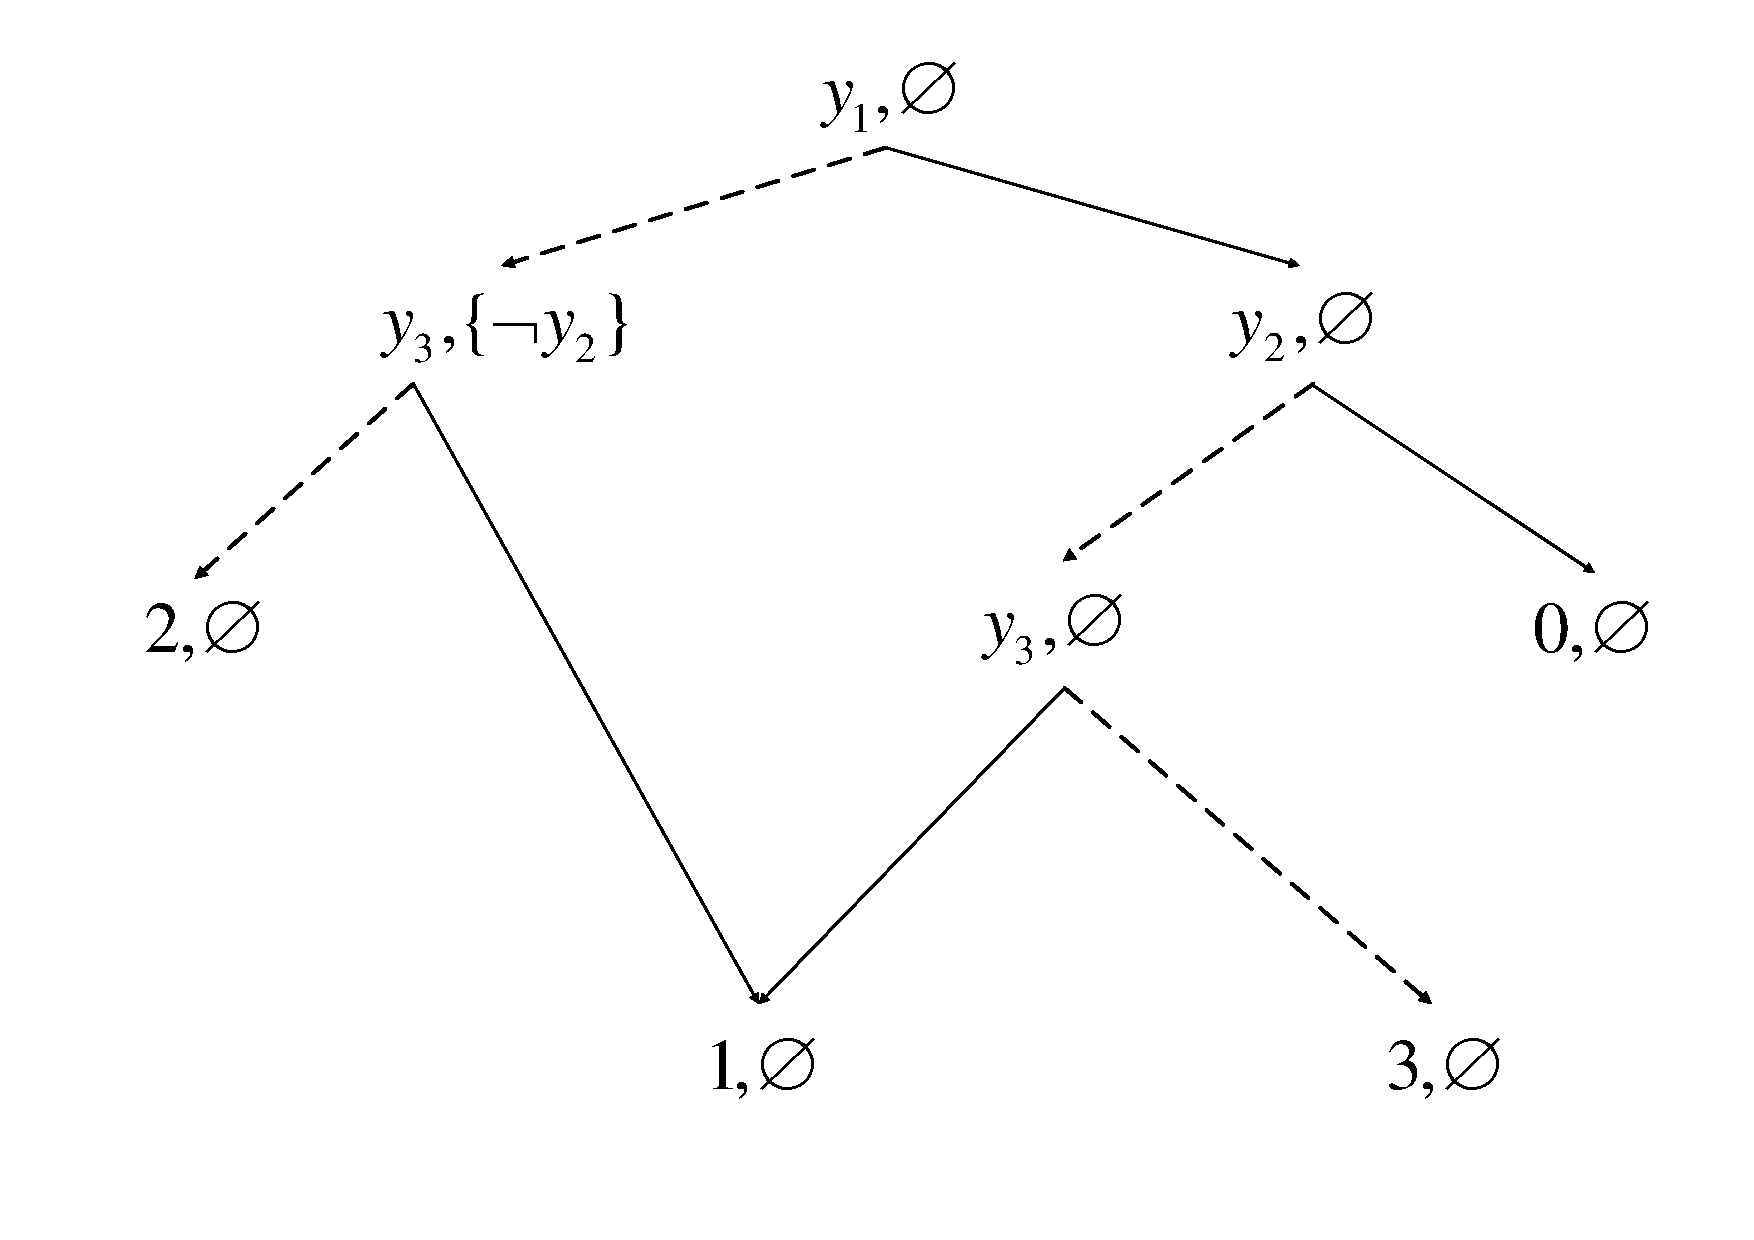
\includegraphics[width=0.7\linewidth]{figures/ADD-L-example1.pdf}
	\caption{An ADD-L example corresponding to Example \ref{circuit-example}, where the weight of a terminal node is the model count of $\varphi[\sigma]$ ($\sigma$ is a partial assignment corresponding to the decisions on a path from the root to it)}
	\label{fig:ADDL-example1}
\end{figure}

\subsection{Tractable Computation of Weight and Entropy}
	%\left| \mathit{Sol}(\varphi(Y \mapsto \sigma)) \right| & \text{$u$ is terminal node and $\sigma \models L(u)$} \\ 
	
	The computation of Shannon entropy of ADD-L depends on the computation of its weight. 
    We first show that for an ADD-L node $u$, we can compute $\omega(u)$ in polynomial time.
	\begin{proposition}\label{prop:omega-proposition}
		Given a non-terminal node $u$ in ADD-L, its weight $\mathit{\omega}(u)$ can be recursively computed as follows in polynomial time:
		$$\mathit{\omega}(u) = 2^{n_0} \cdot \mathit{\omega}(lo(u)) + 2^{n_1} \cdot \mathit{\omega}(hi(u))$$
		where $n_0 = |\mathit{Vars}(u)| - |\mathit{Vars}(lo(u))|-1 - |L(u)|$ and $n_1 = |\mathit{Vars}(u)| - |\mathit{Vars}(hi(u))|-1 - |L(u)|$. 
		%The model counting of the formula represented by $u$ satisfies $CT(u) = \mathit{\omega}(u)$.
		
		\begin{proof}
            The time complexity is immediate by using dynamic programming.
            We prove the equation can compute the weight correctly by induction on the number of variables of the ADD-L rooted at $u$.
            It is obvious that the weight of a terminal node is the real value labeled. 
            Assume that when $|\mathit{Vars}(u)| \le n$, this proposition holds. 
            For the case where $|\mathit{Vars}(u)| = n + 1$, we use $Y_0$ and $Y_1$ to denote $\mathit{Vars}(lo(u))$ and $\mathit{Vars}(hi(u))$, and we have $|Y_0| \le n$ and $|Y_1| \le n$.
            Thus, $\mathit{\omega}(lo(u))$ and $\mathit{\omega}(hi(u))$ can be computed correctly.
            According to Definition \ref{def:ADDL-weight}, $w(u) = \sum_{\sigma \in 2^{\mathit{Vars}(u)}}\omega(\sigma,u)$.
            The assignments over $\mathit{Vars}(u)$ can be divided into three categories: 
            \begin{itemize}
              \item The assignment $\sigma \not\models L(u)$: $\omega(\sigma, u) = 0$.
              \item The assignment $\sigma \models L(u) \cup \{\lnot \mathit{var}(u)\}$: 
              It is obvious that $\omega(\sigma, u) = \omega(\sigma_{\downarrow Y_0}, lo(u))$. 
              Each assignment over $Y_0$ can be extended to exactly $2^{n_0}$ different assignments over $\mathit{Vars}(u)$ in this category. Thus, we have the following equation:
              $$\sum_{\sigma \in 2^{\mathit{Vars}(u)} \land \sigma \models L(u) \cup \{\lnot \mathit{var}(u)\}}\omega(\sigma, u) = 2^{n_0} \cdot \mathit{\omega}(lo(u)).$$
              \item The assignment $\sigma \models L(u) \cup \{\mathit{var}(u)\}$: This case is similar to the above case.
            \end{itemize}
            To sum up, we can obtain that $\mathit{\omega}(u) = 2^{n_0} \cdot \mathit{\omega}(lo(u)) + 2^{n_1} \cdot \mathit{\omega}(hi(u))$.	
		\end{proof}
		
	\end{proposition}
	
	Now we explain how ADD-L computes its Shannon entropy in polynomial time.
	\begin{proposition}\label{prop:Entropy-proposition}
		Given an ADD-L rooted at $u$, we use $\mathit{infor}(v)$ to denote the self-information of the subgraph rooted at $v$.
		We can recursively compute $\mathit{infor}(v)$ in polynomial time as follows:
		\begin{equation*}
		\mathit{infor}(v) =  
		\begin{cases}  
			-\frac{\omega(v)}{\omega(u)} \cdot \log \frac{\omega(v)}{\omega(u)} & v \ is \ terminal   \\
			2^{n_0} \cdot \mathit{infor}(lo(u)) + 2^{n_1} \cdot \mathit{infor}(hi(u)) & otherwise
			
			%-\frac{\omega(v)}{\omega(u)} \cdot \log \frac{\omega(v)}{\omega(u)} \cdot 2^{|Vars(u)| - |Vars(v)|} & v \ is \ terminal   \\
			%\frac{\mathit{infor}(lo(u)) + \mathit{infor}(hi(u))}{2^{ |L(u)| + 1}} & otherwise
			
		\end{cases}  
		\end{equation*}
        where $n_0 = |\mathit{Vars}(v)| - |\mathit{Vars}(lo(v))|-1 - |L(v)|$ and $n_1 = |\mathit{Vars}(v)| - |\mathit{Vars}(hi(v))|-1 - |L(v)|$.  
        The entropy of the probability distribution represented by $u$ satisfies $H(u) = \mathit{infor}(u)$.
		
		
		\begin{proof}
        According to Proposition \ref{prop:omega-proposition}, $\omega(u)$ can be computed in polynomial time, and therefore the time complexity in this proposition is obvious.
		According to Definition \ref{def:ADDL-weight}, $H(u) = -\sum_{\sigma \in 2^{\mathit{Vars}(u)}}\frac{\omega(\sigma,u)}{\omega(u)}\log\frac{\omega(\sigma,u)}{\omega(u)}$.
		We modify the weight of each terminal node $v$ in the ADD-L rooted at $u$ as $-\frac{\omega(v)}{\omega(u)} \cdot \log \frac{\omega(v)}{\omega(u)}$ and assume that the root of the new ADD-L is $u'$.
        It is obvious that $\omega(u') = \mathit{infor}(u)$.
        According to Proposition \ref{prop:omega-proposition}, we know the equation in this proposition can compute $\omega(u')$ correctly.
        Then this proposition holds due to the fact $H(u) = \omega(u')$.
		\end{proof}
		
	\end{proposition}
	
We close this section by explaining why we use the orderedness in the design of ADD-L.
Actually, Propositions \ref{prop:omega-proposition}--\ref{prop:Entropy-proposition} still hold when we only use the more general read-once property: each variable appears at most once in each path from the root of an ADD-L to a terminal node.
First, we observed in our experiments that the linear ordering given by minfill in our tool PSE works better than the dynamic orderings in the state-of-the-art model counters, where the former imposes the orderedness and the latter imposes the read-once property.
Second, ADD-L can provide tractable equivalence checking between probability distributions beyond this study.


\section{PSE: Scalable Precise Entropy Computation}
\label{sec:PSE}

In this section, we introduce our computational tool, PSE, designed to calculate the Shannon entropy of a specified circuit CNF formula with respect to its output variables.
%Just like other Shannon entropy tools, the computing process of PSE is divided into two stages: $Y$-stage (corresponding to outputs) and $X$-stage (corresponding to inputs).
Similar to other Shannon entropy tools, the main process of PSE is divided into two stages: the $Y$-stage (corresponding to outputs) and the $X$-stage (corresponding to inputs).
In the $Y$-stage, we execute a targeted search within the ADD-L framework to accurately compute the Shannon entropy.%File: anonymous-submission-latex-2025.tex
\documentclass[letterpaper]{article} % DO NOT CHANGE THIS
\usepackage[submission]{aaai25}  % DO NOT CHANGE THIS
\usepackage{times}  % DO NOT CHANGE THIS
\usepackage{helvet}  % DO NOT CHANGE THIS
\usepackage{courier}  % DO NOT CHANGE THIS
\usepackage[hyphens]{url}  % DO NOT CHANGE THIS
\usepackage{graphicx} % DO NOT CHANGE THIS
\urlstyle{rm} % DO NOT CHANGE THIS
\def\UrlFont{\rm}  % DO NOT CHANGE THIS
\usepackage{natbib}  % DO NOT CHANGE THIS AND DO NOT ADD ANY OPTIONS TO IT
\usepackage{caption} % DO NOT CHANGE THIS AND DO NOT ADD ANY OPTIONS TO IT
\frenchspacing  % DO NOT CHANGE THIS
\setlength{\pdfpagewidth}{8.5in} % DO NOT CHANGE THIS
\setlength{\pdfpageheight}{11in} % DO NOT CHANGE THIS
%
% These are recommended to typeset algorithms but not required. See the subsubsection on algorithms. Remove them if you don't have algorithms in your paper.
%\usepackage{algorithm}
%\usepackage{algorithmic}


\usepackage{amsmath} 
\usepackage{amsthm}
\newtheorem{example}{Example}[section]
\newtheorem{proposition}{Proposition}[section]
\newtheorem{definition}{Definition}[section]
\usepackage[ruled,vlined]{algorithm2e}
\usepackage{comment}

\usepackage{graphicx}
\usepackage{booktabs}
\usepackage{multirow}


%
% These are are recommended to typeset listings but not required. See the subsubsection on listing. Remove this block if you don't have listings in your paper.
\usepackage{newfloat}
\usepackage{listings}
\DeclareCaptionStyle{ruled}{labelfont=normalfont,labelsep=colon,strut=off} % DO NOT CHANGE THIS
\lstset{%
	basicstyle={\footnotesize\ttfamily},% footnotesize acceptable for monospace
	numbers=left,numberstyle=\footnotesize,xleftmargin=2em,% show line numbers, remove this entire line if you don't want the numbers.
	aboveskip=0pt,belowskip=0pt,%
	showstringspaces=false,tabsize=2,breaklines=true}

%
% Keep the \pdfinfo as shown here. There's no need
% for you to add the /Title and /Author tags.
\pdfinfo{
	/TemplateVersion (2025.1)
}

% DISALLOWED PACKAGES
% \usepackage{authblk} -- This package is specifically forbidden
% \usepackage{balance} -- This package is specifically forbidden
% \usepackage{color (if used in text)
	% \usepackage{CJK} -- This package is specifically forbidden
	% \usepackage{float} -- This package is specifically forbidden
	% \usepackage{flushend} -- This package is specifically forbidden
	% \usepackage{fontenc} -- This package is specifically forbidden
	% \usepackage{fullpage} -- This package is specifically forbidden
	% \usepackage{geometry} -- This package is specifically forbidden
	% \usepackage{grffile} -- This package is specifically forbidden
	% \usepackage{hyperref} -- This package is specifically forbidden
	% \usepackage{navigator} -- This package is specifically forbidden
	% (or any other package that embeds links such as navigator or hyperref)
	% \indentfirst} -- This package is specifically forbidden
% \layout} -- This package is specifically forbidden
% \multicol} -- This package is specifically forbidden
% \nameref} -- This package is specifically forbidden
% \usepackage{savetrees} -- This package is specifically forbidden
% \usepackage{setspace} -- This package is specifically forbidden
% \usepackage{stfloats} -- This package is specifically forbidden
% \usepackage{tabu} -- This package is specifically forbidden
% \usepackage{titlesec} -- This package is specifically forbidden
% \usepackage{tocbibind} -- This package is specifically forbidden
% \usepackage{ulem} -- This package is specifically forbidden
% \usepackage{wrapfig} -- This package is specifically forbidden
% DISALLOWED COMMANDS
% \nocopyright -- Your paper will not be published if you use this command
% \addtolength -- This command may not be used
% \balance -- This command may not be used
% \baselinestretch -- Your paper will not be published if you use this command
% \clearpage -- No page breaks of any kind may be used for the final version of your paper
% \columnsep -- This command may not be used
% \newpage -- No page breaks of any kind may be used for the final version of your paper
% \pagebreak -- No page breaks of any kind may be used for the final version of your paperr
% \pagestyle -- This command may not be used
% \tiny -- This is not an acceptable font size.
% \vspace{- -- No negative value may be used in proximity of a caption, figure, table, section, subsection, subsubsection, or reference
% \vskip{- -- No negative value may be used to alter spacing above or below a caption, figure, table, section, subsection, subsubsection, or reference

\setcounter{secnumdepth}{0} %May be changed to 1 or 2 if section numbers are desired.

% The file aaai25.sty is the style file for AAAI Press
% proceedings, working notes, and technical reports.
%

% Title

% Your title must be in mixed case, not sentence case.
% That means all verbs (including short verbs like be, is, using,and go),
% nouns, adverbs, adjectives should be capitalized, including both words in hyphenated terms, while
% articles, conjunctions, and prepositions are lower case unless they
% directly follow a colon or long dash
\title{Scalable Precise Computation of Shannon Entropy}
\author{
%Authors
% All authors must be in the same font size and format.
Written by AAAI Press Staff\textsuperscript{\rm 1}\thanks{With help from the AAAI Publications Committee.}\\
AAAI Style Contributions by Pater Patel Schneider,
Sunil Issar,\\
J. Scott Penberthy,
George Ferguson,
Hans Guesgen,
Francisco Cruz\equalcontrib,
Marc Pujol-Gonzalez\equalcontrib
}
\affiliations{
%Afiliations
\textsuperscript{\rm 1}Association for the Advancement of Artificial Intelligence\\
% If you have multiple authors and multiple affiliations
% use superscripts in text and roman font to identify them.
% For example,

% Sunil Issar\textsuperscript{\rm 2},
% J. Scott Penberthy\textsuperscript{\rm 3},
% George Ferguson\textsuperscript{\rm 4},
% Hans Guesgen\textsuperscript{\rm 5}
% Note that the comma should be placed after the superscript

1101 Pennsylvania Ave, NW Suite 300\\
Washington, DC 20004 USA\\
% email address must be in roman text type, not monospace or sans serif
proceedings-questions@aaai.org
%
% See more examples next
}

%Example, Single Author, ->> remove \iffalse,\fi and place them surrounding AAAI title to use it
\iffalse
\title{My Publication Title --- Single Author}
\author {
Author Name
}
\affiliations{
Affiliation\\
Affiliation Line 2\\
name@example.com
}
\fi

\iffalse
%Example, Multiple Authors, ->> remove \iffalse,\fi and place them surrounding AAAI title to use it
\title{My Publication Title --- Multiple Authors}
\author {
% Authors
First Author Name\textsuperscript{\rm 1},
Second Author Name\textsuperscript{\rm 2},
Third Author Name\textsuperscript{\rm 1}
}
\affiliations {
% Affiliations
\textsuperscript{\rm 1}Affiliation 1\\
\textsuperscript{\rm 2}Affiliation 2\\
firstAuthor@affiliation1.com, secondAuthor@affilation2.com, thirdAuthor@affiliation1.com
}
\fi


% REMOVE THIS: bibentry
% This is only needed to show inline citations in the guidelines document. You should not need it and can safely delete it.
\usepackage{bibentry}
% END REMOVE bibentry



\begin{document}


% Uncomment the following to link to your code, datasets, an extended version or similar.
%
% \begin{links}
	%     \link{Code}{https://aaai.org/example/code}
	%     \link{Datasets}{https://aaai.org/example/datasets}
	%     \link{Extended version}{https://aaai.org/example/extended-version}
	% \end{links}


\begin{abstract}
	Quantitative information flow analyses (QIF) are a class of techniques for measuring the amount of confidential information leaked by a program to its public outputs. 
	Shannon entropy is an important method to quantify the amount of leakage in QIF.
	This paper focuses on the programs modeled in Boolean clausal constraints and optimises the two stages of the Shannon entropy computation to implement a scalable precise tool PSE.
	In the first stage, we design a knowledge compilation language called ADD-L that combines Algebraic Decision Diagrams and implied Literals.
	ADD-L avoids enumerating possible outputs of a program and supports tractable entropy computation. 
	In the second stage, we optimise the model counting queries that are used to compute the probabilities of outputs. 
	We evaluate the performance of PSE, and the experiments demonstrate that PSE significantly enhances the scalability of precise entropy computation and even outperforms the state-of-the-art approximate tool EntropyEstimation.
\end{abstract}





\input{Sections/1.tex}

\input{Sections/2-Notations and Background.tex}

\input{Sections/3-Algebraic Decision Diagram With Implied Literals.tex}

\input{Sections/4-PSE An precise entropy solver.tex}

\input{Sections/5-Experiments.tex}

\input{Sections/6-Related work.tex}

\input{Sections/7-Conclusions.tex}


\bibliography{references}
\end{document}

In the $X$-stage, we perform multiple optimized model counting.
PSE, depicted in Algorithm \ref{PSE}, takes in a CNF formula $\varphi$, an input set $X$, and an output set $Y$, and returns the self-information $\mathit{infor}(\sigma, \varphi)$ of the formula, where $\sigma$ is the assignment made in the ancestor calls.
As mentioned in Proposition \ref{prop:Entropy-proposition}, the entropy of the original formula is the output of the root call.


\begin{algorithm}[h]
	\caption{PSE($\varphi$,$X$,$Y$)}
	\label{PSE}
	\LinesNumbered
    \DontPrintSemicolon
	\KwIn{A circuit CNF formula $\varphi$ with inputs $X$ and outputs $Y$}
	\KwOut{the self-information of $\varphi$}
	\lIf{$\varphi = \mathit{false}$} {\Return $0$}
	
	%\If{$\varphi = \mathit{true}$}  { $p \leftarrow 2^{|\varphi| - |Y|}$ \Return $2^{|Y|} \cdot (-p \cdot \log p) $\}
	$n \leftarrow |\mathit{Vars}(\varphi)|$
	
	$L \leftarrow \texttt{GetImpliedLiterals}(\varphi)$ 
	
	$\varphi,Y \leftarrow $\texttt{Simplify}($\varphi, Y, L$) 
	
	\lIf{$\mathit{Cache}(\varphi) \neq nil $} {\Return $\mathit{Cache}(\varphi)$}
	\If{$ Y = \emptyset $}
	{
		$m \leftarrow $ \texttt{CountModels}($\Phi$) 
		
		$p \leftarrow \frac{m}{TotalCount} $
		
		%$\mathit{infor} \leftarrow -p \cdot \log {p}$
		
		\Return  $Cache(\varphi)  \leftarrow 
		-p \cdot \log {p}$
		%\texttt{\mathit{infor}Computing}($\varphi$) $\cdot 2^{|V| - | Vars(\varphi) |}$	
	}
	$ y \leftarrow \texttt{PickGoodVar}(Y)$
	
	$ \varphi_0 \leftarrow \varphi[y \mapsto \mathit{false}]$
	
	$ \varphi_1 \leftarrow  \varphi[y \mapsto \mathit{true}]$
	
	$\mathit{infor}_0 \leftarrow $ PSE($\varphi_0,X,Y \backslash y$)
	
	$\mathit{infor}_1 \leftarrow $  PSE($\varphi_1,X,Y \backslash y$) 
	
	\Return $\mathit{Cache}(\varphi)  \leftarrow $ $2^{n - |\mathit{Vars}(\varphi_0)| - |L| - 1} \cdot  \mathit{infor}_0 +  2^{n - |\mathit{Vars}(\varphi_1)| - |L| - 1} \cdot \mathit{infor}_1$
	%\Return $Cache(\varphi)  \leftarrow \frac{infor_f + infor_t}{2^{|L| + 1}}$
	
\end{algorithm}

We first deal with the cases in which $\varphi$ is $\mathit{false}$ in line 1.  
In such instances where the formula $\varphi$ evaluates to $\mathit{false}$, the self-information associated with the assignment from the ancestor calls is defined as 0.
%When the formula $\varphi$ is $\mathit{true}$, we use a simplification technique where for the remaining unassigned variables $Y$, there are a total of $2^Y$ satisfying assignments.  Therefore, we have $2^{|Y|}$ terminal nodes with a weight of $2^{|\varphi|-|Y|}$ each.
In line 2, we record the number of variables in $\varphi$. 
Subsequently, in line 3, we utilize the \texttt{GetImpliedLiterals} function to extract the implied literals of $\varphi$.
The implementation of \texttt{GetImpliedLiterals} relies on implicit Boolean Constraint Propagation (i-BCP)~\cite{thurley2006sharpsat}. 
In line 4, we simplify both the formula $\varphi$ and the set $Y$ utilizing the extracted implied literals $L$.
Detect whether the simplified formula $\varphi$ has been stored  in the cache in line 5, and return its $\mathit{infor}$ if $\varphi$ hits the cache.
If the current $Y$ is an empty set (in line 6), it means that a satisfiable assignment under the restriction of the output set $Y$ has been obtained. 
We do not explicitly address the case where $\varphi$ evaluates to $\mathit{true}$, as this naturally results in set $Y$ being empty—a defining trait of circuit formulas.
Consequently, the scenario where set $Y$ is empty inherently includes the case where $\varphi$ is $\mathit{true}$.
Lines 7--9 query model counting for the residual formula and calculate its $\mathit{infor}$, corresponding to the terminal case of proposition \ref{prop:Entropy-proposition}.
$TotalCount$ represents the total number of models for the original formula, i.e., for the original formula $\varphi$, $TotalCount= |\mathit{Sol}(\varphi)|$. 
This value is obtained directly through the invocation of any model counter before PSE.
In line 9, the computed self-information $\mathit{infor}$ is cached and then returned as the final result.
If any remaining variables in $Y$ have not been assigned values, we make decisions about them in line 10.
The \texttt{PickGoodVar} function operates as a heuristic algorithm designed to select a variable from set $Y$, with the selection criteria being determined by the specific heuristic employed.
Moving forward, lines 11 and 12 are dedicated to generating the residual formulas $\varphi_0$ and $\varphi_1$, which correspond to the scenarios where the variable $y$ is assigned the values $\mathit{false}$ and $\mathit{true}$, respectively. Following this, lines 13 and 14 are utilized to recursively determine the self-information $\mathit{infor}$ for each of these derived formulas.
Since $\varphi$ is a circuit formula, all residual formulas in the recursive process after the variables in decision $Y$ are also circuit formulas.
Finally, we compute the information for $\varphi$ (corresponding to the non-terminal case of proposition \ref{prop:Entropy-proposition}) and store it in the cache, returning it as the result in line 15.


\subsection{Implementation}

We now discuss the implementation details that are crucial for the runtime efficiency of PSE. 
Specifically, leveraging the tight interplay between entropy computation and model counting, our methodology integrates a variety of state-of-the-art techniques in model counting.

Initially, we have the option to employ various methodologies for the model counting query denoted by \texttt{CountModels} at line 7.
The first considered method is to individually employ state-of-the-art model counters, such as SharpSAT-TD \cite{korhonen2021integrating}, Ganak~\cite{sharma2019ganak}, ExactMC~\cite{lai2021power}, and D4~\cite{lagniez2017improved}.
The second method, called \textbf{ConditionedCounting}, requires the prior construction of a representation of the original formula $\varphi$ to support tractable model counting.
This method is compatible with eligible representation languages such as d-DNNF~\cite{darwiche2004new}, OBDD[$\land$]~\cite{lai2017new}, and SDD~\cite{choi2013compiling}.
Upon reaching line 7, the algorithm executes conditioned model counting, utilizing the compiled representation of the formula and incorporating the partial assignment derived from the ancestor calls.
The last method, called \textbf{SharedCounting}, also solves model counting query by invoking the exact model counter.
Distinct from the first method, \textbf{SharedCounting} does not merely perform model counting in isolation.
Instead, it leverages a shared component cache within the counter across all model counting queries, a strategy we term \textbf{XCache}.
To distinguish it from the cache method in the $X$-stage, we refer to the cache method in the $Y$-stage as \textbf{YCache} in the following.
To differentiate it from the caching approach used in the $X$-stage, the caching method employed in the $Y$-stage is referred to as \textbf{YCache}.
Our observations indicate that the \textbf{SharedCounting} method is most effective within the PSE framework.

\begin{figure}[!htbp]
	
	\centering
	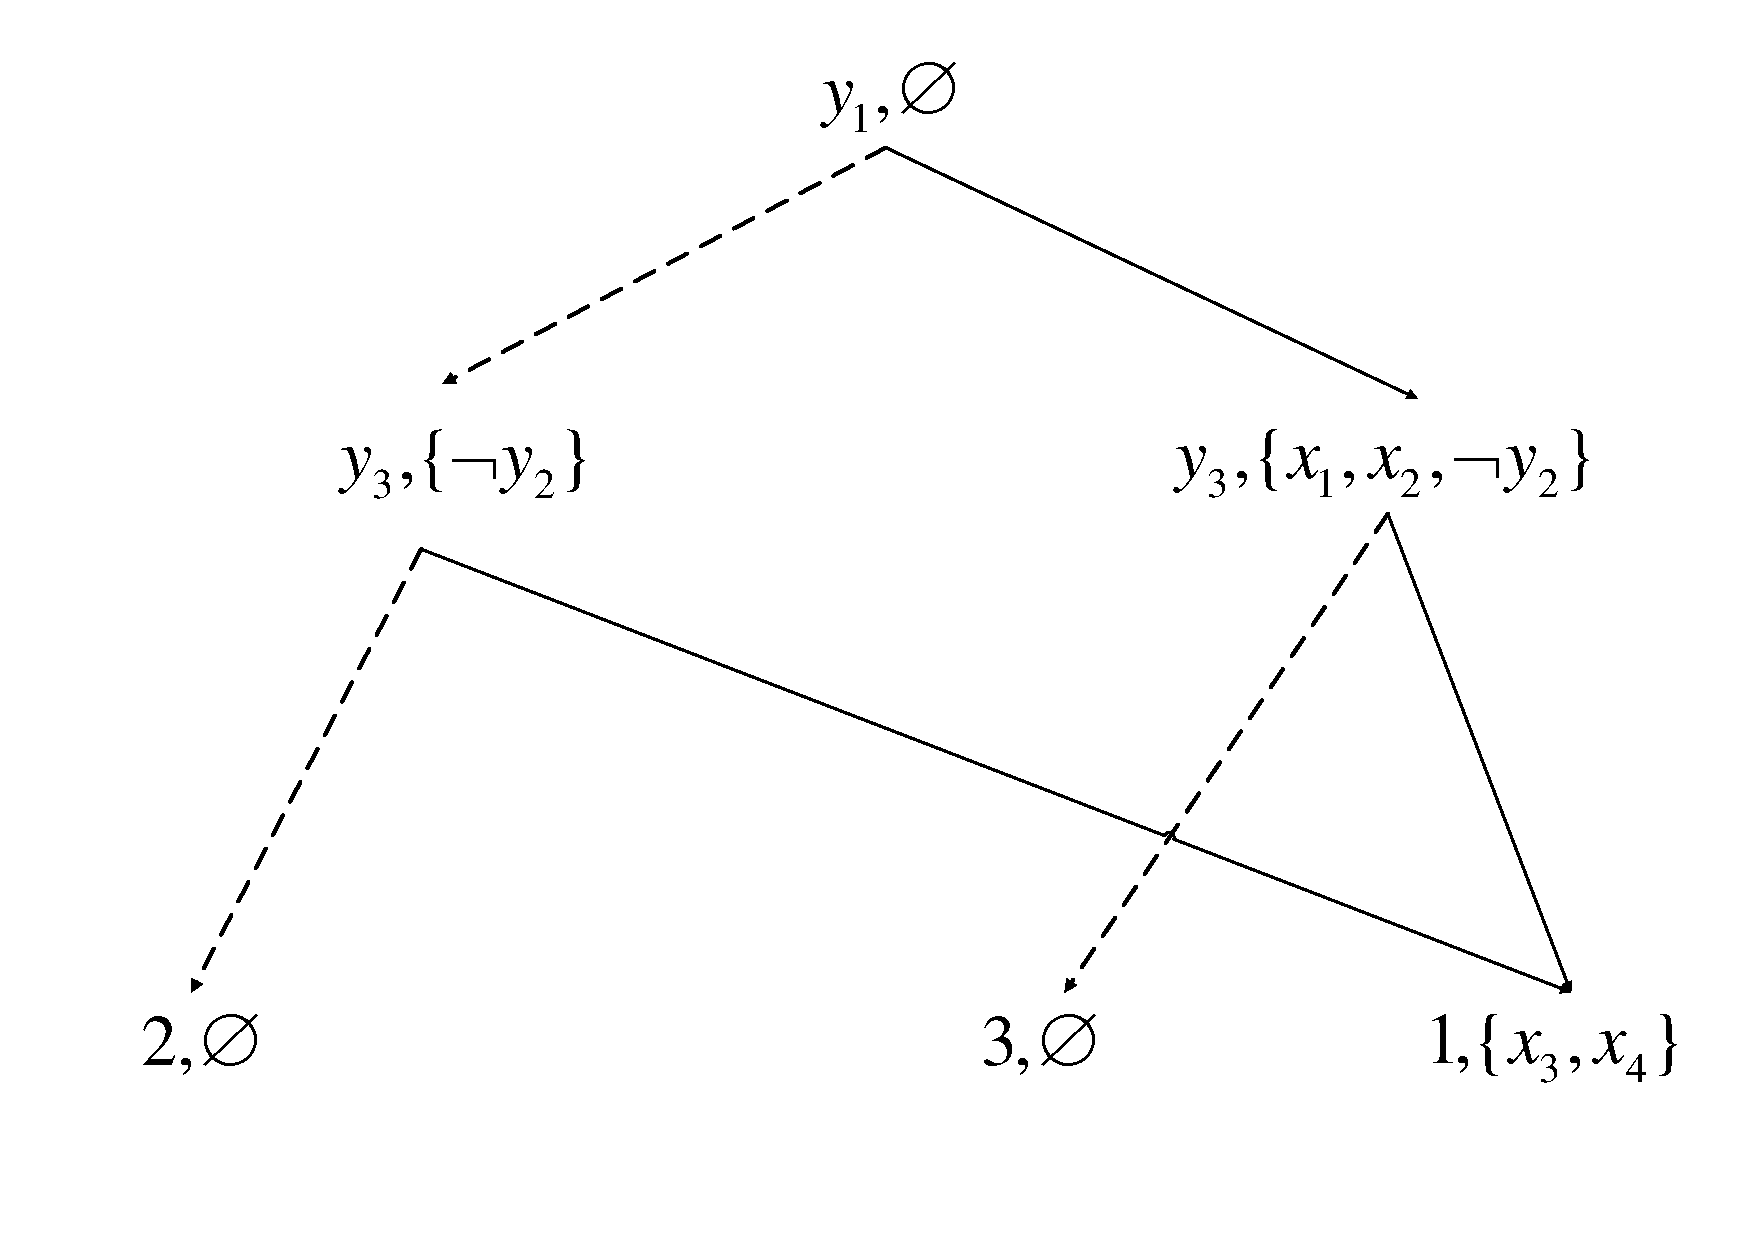
\includegraphics[width=0.7\linewidth]{figures/ADD-L-example2.pdf}
	\caption{An ADD-L example corresponding to Example \ref{circuit-example}, where the implied literals include the variables in $X$. }
	\label{fig:ADDL-example2}
\end{figure} 

\textbf{Implied Literal}
According to the definition of entropy, the assignment $\sigma$ is confined to the variables in set $Y$, implying that, in theory, the implied literals should exclusively involve variables that belong to $Y$.
%However, we observed that if the implied literals are not restricted to only variables in $Y$ and can also include variables in $X$, it can further simplify the formula and optimize the structure of ADD-L.
However, our observations indicate that the ADD-L structure can achieve further simplification and optimization if it is not constrained to implied literals involving only variables in $Y$, but is allowed to encompass variables in $X$ as well.
In light of this insight, we implemented enhancements to the computation of implied literals by lifting the constraints, thus permitting the inclusion of variables from set $X$.
Furthermore, we discovered that employing this technique augments the search efficiency while maintaining the precision of the entropy computation.
To demonstrate the validity and efficacy of this approach, we present an illustrative example in Figure \ref{fig:ADDL-example2}.
%It is easy to see from the comparison between Figure \ref{fig:ADDL-example2} and Figure \ref{fig:ADDL-example1} that this approach optimizes the structure of ADD-L without affecting the entropy result.
A comparison between Figure \ref{fig:ADDL-example1} and Figure \ref{fig:ADDL-example2} clearly demonstrates that the approach successfully optimizes the ADD-L structure without affecting the accuracy of the computed entropy.


\textbf{Variable Decision Heuristic} 
We implement the current state-of-the-art model counting heuristics for the Shannon entropy computation problem and conduct comparative experiments, encompassing \textbf{VSADS}~\cite{sang2005heuristics}, \textbf{minfill}~\cite{darwiche2009modeling}, the \textbf{SharpSAT-TD} heuristic~\cite{korhonen2021integrating}, and \textbf{DLCP}~\cite{lai2021power}.
Through our experimentation with various heuristics, the results consistently indicate that the minfill heuristic achieves superior performance in addressing the entropy computation problem.
Consequently, we adopt the \textbf{minfill} heuristic as the default for our subsequent experiments.

\textbf{Preprocessing} 
%Since the core of entropy computing is model counting, we try to integrate the preprocessing strategy in model counting into our entropy tool PSE.
%Based on Literal Equivalences, which is a powerful technique in SAT solving, we implement a new preprocessing approach in PSE.
Recognizing that model counting lies at the heart of entropy computation, we have enhanced our entropy tool, PSE, by incorporating an advanced preprocessing technique that capitalizes on literal equivalence in model counting. 
This idea is inspired by the work of Lai et al. \cite{lai2021power} on capturing literal equivalence in knowledge compilation.
However, due to the specific nature of the entropy computation process, it is not feasible to arbitrarily replace the literals corresponding to variables in the output set with their equivalents.
%This is because the new formula $\varphi '$ obtained after the equivalent substitution of literals is equivalent to $\varphi$ in model counting, but not necessarily equivalent in entropy (it is not equivalent when the variables corresponding to the substituted literals belong to $Y$).
%At the beginning, we had a simple idea to restore all equivalent literals after the calculation, in order not to affect the calculation of the entropy and at the same time to reduce the size of the formula.
This is because the new formula $\varphi'$ obtained after the equivalent substitution of literals is equivalent to $\varphi$ in model counting, but not necessarily equivalent in entropy (it is not equivalent when the variables of substituted literals belong to $Y$).
In the beginning, we had the simple idea of restoring all equivalent literals after the calculation so as not to affect the calculation of the entropy and, at the same time, reduce the size of the formula.
We improve this idea by restoring only the literals corresponding to the variables in $Y$, since the assignments that affect the entropy are only in the part of $Y$. 
The new preprocessing method is called \textbf{Pre} in the following.
Experiments have demonstrated that this preprocessing method provides some performance enhancement to the tool (See Section \ref{sec:Experiments}).
This idea of preprocessing is motivated by the fact that, on the one hand, after preprocessing using literal equivalence, it can simplify the formula and thereby improve the efficiency of the subsequent model counting.
On the other hand (and more importantly), it reduces the treewidth of the tree decomposition, which leads to a more optimal order of variable selection obtained by the tree decomposition heuristic, and can be very effective in improving the efficiency of PSE calculations.




\begin{comment}
	Algorithm \ref{Condition} describes another model counting method in $X$-stage.
	To implement this method, a prerequisite is that we need an ADD-L constructed based on the original minfill static variable order. The difference between this ADD-L and the ADD-L corresponding to Algorithm 2 is that the $Y$-stage of Algorithm 2 is equivalent to making decisions only on the variables of the $Y$ set based on the minfill static variable order, while our new idea is to make decisions on all variables in the order of the minfill static variable order (including var in $X$). 
	The motivation for this is that our experiments have found that the heuristic effect of the minfill linear order is much stronger (making decisions only on the variables of the $Y$ set to some extent disrupts the linear order). 
	At this point, the computing process is more like general model counting, which can efficiently construct ADD-L. 
	With such an ADD-L, we can utilize conditional model counting (or entropy computing) in knowledge compilation to solve the model counting in the $X$-stage. 
	Lines 1-2 of the algorithm indicate that when the result of a node hits the cache, we can directly retrieve the corresponding result from the cache. 
	When accessing a terminal node, we directly return the result of the corresponding terminal node (lines 4-5). 
	If the variable decision of node u is false, we recursively call the lo branch to solve it (lines 7-8). 
	Similarly, when the variable decision of node u is true, we recursively call the hi branch to solve it (lines 10-11). Otherwise, it means that the variable corresponding to the node has not been decided, so both lo and hi need to be called (line 13). 
	We cache the current result and return it in lines 14-15.
	
	
	
	If any remaining variables in $Y$ have not been assigned values, we make decisions about them in lines 8-10.
	First, a variable x is chosen heuristically.
	Next the $infor$ of the subformula is computed recursively for two different values (true, false) of $x$. 
	Finally, the $infor$ of the two subformulas ($\varphi[y \mapsto false]$ and $\varphi[y \mapsto true]$) are summed to obtain the $infor$ of the current formula, and the $infor$ associated with the corresponding formula is added to the cache.
	
	Whenever we obtain a satisfiable assignment $\sigma_{\downarrow Y}$ under the restriction of the output set $Y$, we need to calculate the number of different inputs corresponding to this assignment.
	This step can be achieved by performing model counting on the remaining formulas (corresponding to the numerator of $p_{\sigma}$).
	According to \ref{projected-proposition},  the denominator of  $p_{\sigma}$ can be represented by the total number of models of $\varphi$, from which $p_{\sigma}$ can be calculated, and then the $infor$ of the sub-formula can be derived.
	Algorithm \ref{InforComputing} describes this process. 
	
	Algorithm \ref{InforComputing} receives a remaining CNF formula $\Phi$ after all variables in $Y$ have been assigned and returns the $infor$ $H(\varphi)$ of $\Phi$.
	As mentioned above, we perform model counting on the remaining sub-formulas in lines 1-4.
	In the model counting of the $X$-stage, we propose two methods, called \textbf{Counting} and \textbf{Condition}, with $count_{opt}$ as a parameter to indicate the chosen method.
	The first approach corresponds to lines 1-2, where any exact model counting tool can be called. 
	It's worth noting that this method does not just query the model counting individually.
	Instead, we share the component cache for all model counting queries, and we refer to this strategy as \textbf{XCache}.
	The other method requires constructing in advance an ADD-L that contains all the variables in $Y$, which can also include variables from the $X$.
	Then convert the model counting into conditional model~\cite{lai2017new} counting based on the current variable assignment.
	In line 5, probability $p_{\sigma}$ is computed according to the definition in Section 2, where $totalcount$ is the number of models of the entire formula $\varphi$, which is also computed by a model counting tool. 
	We only need to calculate $totalcount$ once and store it. 
	In line 6, the $infor$ can be obtained from $p_{\sigma}$ and returned as a result in line 7.
	
\end{comment}



\section{Experiments}
\label{sec:Experiments}

To evaluate the performance of PSE, we implemented a prototype in C++ that employs ExactMC as the model counter.
We evaluate PSE in 361 benchmarks, including the QIF  benchmarks~\cite{fremont2017maximum}, combinatorial circuits, plan recognition~\cite{soos2020tinted}, bit-blasted versions of SMTLIB benchmarks~\cite{sharma2019ganak}, and QBFEval competitions~\cite{golia2022scalable}. %~\cite{qbfeval2017, qbfeval2018}. 
All experiments were run on a computer with Intel(R) Core(TM) i9-10920X CPU @ 3.50GHz and 32GB RAM.
Each instance was run on a single core with a timeout of 3000 seconds and 8GB memory.


Through our evaluations and analysis, we sought to answer the following research questions:
\begin{itemize}
	\item \textbf{RQ1:} How does the runtime performance of PSE compare to the state-of-the-art precise Shannon entropy tools?
	\item \textbf{RQ2:} How does the runtime performance of PSE compare to the state-of-the-art Shannon entropy estimation tool?
	\item \textbf{RQ2:} How do the utilized methods impact the runtime performance of PSE? 
\end{itemize}


\subsection{Comparison with precise Shannon entropy tools}

\begin{table}[h!]
	\centering
	\resizebox{\linewidth}{!}
	{
		\begin{tabular}{ cccccccccc } 
			\toprule 
			\multirow{2}*{instance} & \multirow{2}*{$\left| X \right|$} & \multirow{2}*{$\left| Y \right|$} & \multicolumn{2}{c}{baseline-SharpSAT-TD} & \multicolumn{2}{c}{baseline-ExactMC} & \multicolumn{2}{c}{PSE} \\
			
			\cmidrule(r){4-5}   
			\cmidrule(r){6-7}
			\cmidrule(r){8-9}  
			
			& & & Entropy & Time(s) & Entropy & Time(s) & Entropy & Time(s)\\ 
			
			\midrule  
			blasted$\_$case102.cnf & 11 & 23 & 8 & 81.29 & 8 & 0.39 & 8 & 0.16 \\
			s27$\_$15$\_$7.cnf & 7 & 25 & 3.3 & 142.77  & 3.3 & 0.15 & 3.3 & 0.14 \\
			small-bug1-fixpoint-5.cnf & 66 & 21 & 12.81 & 79.51 & 12.81 & 2.99 & 12.81 & 0.18 \\
			small-bug1-fixpoint-6.cnf & 79 & 25 & 15.31 & 1406.47 & 15.31 & 51.9 & 15.31 & 0.21 \\
			blasted$\_$case144.cnf & 138 & 627 & - & - & - & - & 77.62 & 35.42 \\
			s1423a$\_$15$\_$7.cnf & 91 & 773 & - & - & - & - &  88.17 & 232.65 \\
			s382$\_$15$\_$7.cnf & 24 & 326 & - & - & - & - & 23.58 & 0.22 \\
			CVE-2007-2875.cnf & 752 & 32 & - & - & - & - & 32 & 0.72 \\
			10.sk$\_$1$\_$46.cnf & 47 & 1447 & - & - & - & - & 13.58 & 0.18 \\
			
			\bottomrule
		\end{tabular}
	}
	\caption{Entropy computing performance of baseline and PSE. "-" represents that the entropy cannot be solved within the specified time limit.
	\label{table:1}
	}
\end{table}
The existing precise Shannon entropy tools do not use the techniques in the state-of-the-art model counters.
Just like~\cite{golia2022scalable}, we implemented the precise Shannon entropy baseline with state-of-the-art model counting techniques.
In the baseline, we enumerate each assignment $\sigma \in \mathit{Sol}(\varphi)_{\downarrow Y}$ and compute $p_{\sigma} = \frac{\left| \mathit{Sol}(\varphi(Y \mapsto \sigma)) \right|}{ \left| \mathit{Sol}(\varphi)_{\downarrow X} \right| }$, where $\mathit{Sol}(\varphi(Y \mapsto \sigma))$ denotes the set of solutions of $\varphi(Y \mapsto \sigma)$ and $\mathit{Sol}(\varphi)_{\downarrow X}$ denotes the set of solutions of $\varphi$ projected to $X$.
As can be seen from the previous proposition, $| \mathit{Sol}(\varphi)_{\downarrow X} |$ can be replaced by $| \mathit{Sol}(\varphi) |$.
Finally, entropy is computed as $H(\varphi) = \sum_{\sigma \in 2^Y} -p_{\sigma} \log {p_{\sigma}} $.
For a formula with an output set size of $m$, $2^m$ model counting queries are required, and we chose the state-of-the-art model counters SharpSAT-TD and ExactMC to the model counting queries, respectively.

In our experiment, the baseline with SharpSAT-TD (resp. ExactMC) can only solve 17 instances within the specified time of 3000 seconds, while PSE can solve 289 instances. 
Table \ref{table:1} shows the comparison between baseline and PSE on some instances.
The results show a significant improvement in the efficiency of PSE for computing the precise Shannon entropy, which answers \textbf{RQ1} as well.


\subsection{Comparison with Shannon entropy estimation tool}
We compare PSE with EntropyEstimation, the current state-of-the-art Shannon entropy estimation tool on 361 instances. 
Table \ref{table:2} shows the performance of PSE and EntropyEstimation~\cite{golia2022scalable} in entropy computing.


\begin{table}[h!]
	\centering
	\begin{tabular}{ ccccc } 
		\toprule 
		\multirow{2}{*}{tool}  & \multicolumn{3}{c}{Instances Solved} & \multirow{2}{*}{Average PAR-2 score} \\
		 \cline{2-4}
		& Unique & Fastest & Total \\ 
		\midrule 
		EntropyEstimation & 10 & 0 & 264 & 1574.59 \\ 
		
		PSE & \textbf{35} & \textbf{254} & \textbf{289} & \textbf{1193.37} \\
		\bottomrule
	\end{tabular}
	\caption{Detailed performance comparison of PSE and EntropyEstimation. Unique represents the number of instances that can only be solved by a specific tool. Fastest represents the number of instances that a tool solves with the shortest time.}
	\label{table:2}
\end{table}

\begin{figure}[htbp]
	\centering
	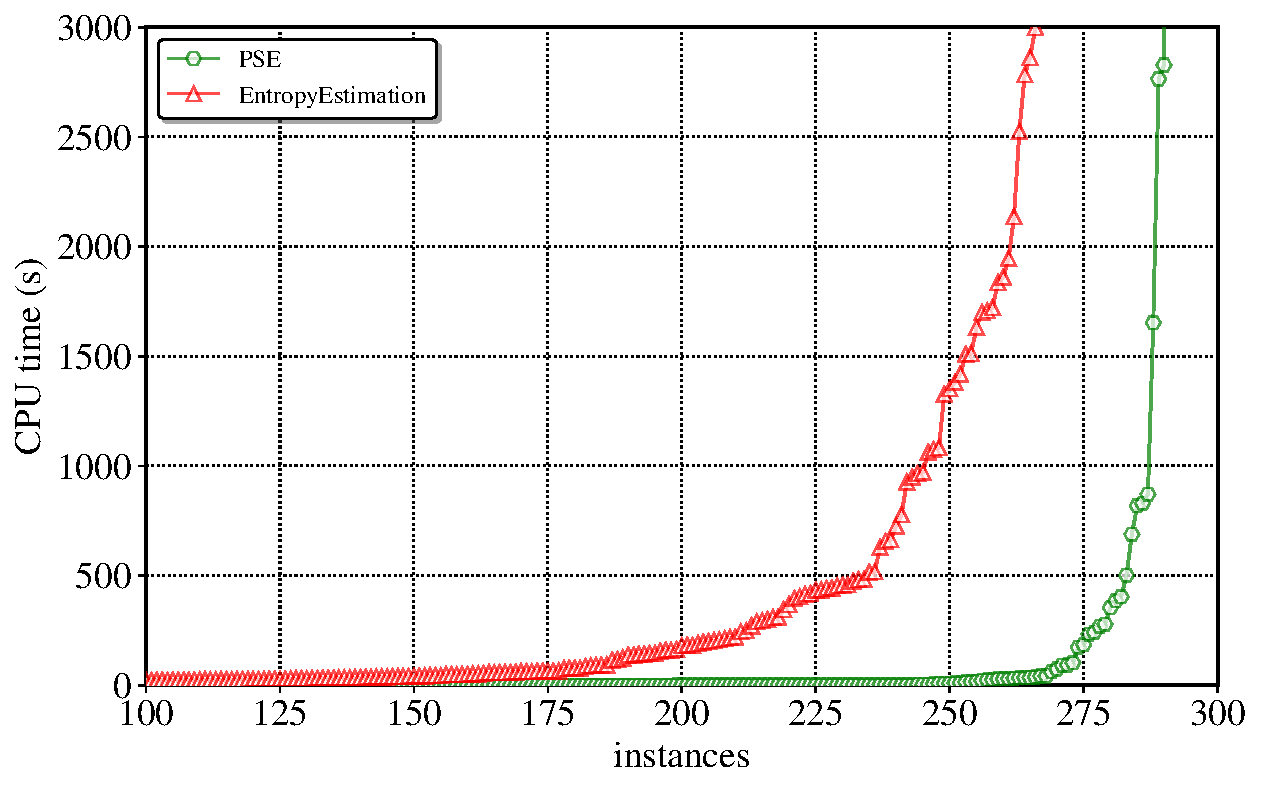
\includegraphics[width=7cm,height=8cm]{figures/PSEvsEntropyEstimation.pdf}
	\caption{Cactus plot comparing the computing time of PSE and EntropyEstimation.
	}
	\label{figure:2}
\end{figure} 

Table \ref{table:2} shows that, among the 361 instances tested and within the 3000-second time limit, our tool PSE successfully solves 25 more instances than EntropyEstimation, indicating overall superior performance.
For instances where both PSE and EntropyEstimation successfully solve the problem within the time limit, PSE demonstrates a shorter computation time and a substantially lower average PAR-2 score~\footnote{The average PAR-2 scoring scheme gives a penalized average runtime, assigning a runtime of two times the time limit for each benchmark that the tool fails to solve} than EntropyEstimation.
Figure \ref{figure:2} shows the cactus plot of runtime for PSE and EntropyEstimation, where the $x$-axis represents the number of benchmarks and the $y$-axis represents the runtime.

Meanwhile, we identified some instances where PSE timed out while EntropyEstimation was able to solve within the time limit.
Our experiments showed that, in cases where PSE was unable to solve the problem, the number of model counting queries escalated to an order of magnitude of ten million, and the entropy was still not computed.
This suggests a potential bottleneck in the computation of precise Shannon entropy. Therefore, more sophisticated techniques are required to accurately compute the entropy for these challenging instances.
We propose that improvements in preprocessing techniques and more effective variable heuristics for entropy computation could represent key breakthroughs.
Nonetheless, it is crucial to recognize that EntropyEstimation is an estimation tool for Shannon entropy and that its results are subject to a certain margin of error.
Our precise Shannon entropy tool, PSE, consistently performs better than entropy estimators across most instances, highlighting that our methods significantly enhance the scalability of precise Shannon entropy computation.
The results clearly indicate that PSE outperforms EntropyEstimation in the majority of instances. This validates a positive answer to \textbf{RQ2}.

%These experimental results show that PSE has significant advantages over both state-of-the-art precise and approximate entropy tools.
%This also provides an affirmative answer to \textbf{RQ1}.


\subsection{Impact of algorithmic configurations}
To better verify the effectiveness of the PSE methods and answer \textbf{RQ3}, we conducted a comparative study on all the utilized methods, including methods for the $Y$-stage: \textbf{Implied Literal}, \textbf{YCache}, \textbf{Pre}, variable decision heuristics(\textbf{minfill}, \textbf{DLCP}, \textbf{SharpSAT-TD heuristic}, \textbf{VSADS}), and methods for the $X$-stage: \textbf{XCache} and \textbf{ConditionedCounting}.
In accordance with the principle of control variables, we conducted ablation experiments to evaluate the effectiveness of each method, ensuring that each experiment differed from the PSE tool by only one method.
The cactus plot for the different methods is shown in Figure \ref{figure:3}, where PSE represents our tool, PSE-wo-Pre means that \textbf{Pre} is turned off in PSE.
PSE-ConditionedCounting indicates that PSE employed the \textbf{ConditionedCounting} method rather than \textbf{SharedCounting} in the $X$-stage.
PSE-wo-XCache indicates that the caching method is turned off in PSE in the $X$-stage. 
PSE-wo-YCache indicates that the caching method is turned off in PSE in the $Y$-stage.
PSE-wo-ImpliedLiteral indicates that PSE does not employ the \textbf{Implied Literal} in the $Y$-stage.
PSE-dynamic-SharpSAT-TD means that PSE replaces the \textbf{minfill} static variable order with the dynamic variable order: the variable decision-making heuristic method of SharpSAT-TD (all other configurations are the same as in PSE, only the variable decision-making heuristic is different).
Similarly, PSE-dynamic-DLCP and PSE-dynamic-VSADS respectively indicate the selection of dynamic heuristic \textbf{DLCP} and \textbf{VSADS}.

As can be seen from the experimental results, the power of implied literal is very strong. 
The effect of caching is also significant, as has been demonstrated in previous studies of knowledge compilation.
Although the effect of preprocessing is not very significant, it can still increase the number of instances solved.
The heuristic strategies minfill and SharpSAT-TD heuristic both performed well, and the results indicate that the static heuristic minfill is more suitable for entropy computing.
In the technique of the $X$-stage, the \textbf{ConditionedCounting} method performs better than \textbf{SharedCounting} without \textbf{XCache}, but not as well as the \textbf{SharedCounting} method.
This comparative experiment indicates that the shared component caching is quite effective.
The biggest advantage of the \textbf{ConditionedCounting} method is that its time complexity is linear~\cite{lai2017new}, although it also has a major disadvantage in that we need to construct an ADD-L based on the static variable order first, which is a process with a large time overhead for more complex problems.
Although the \textbf{ConditionedCounting} method is not the most effective, we believe it is still a promising and scalable method. 
For instances where an ADD-L can be constructed quickly based on the static variable order, the \textbf{ConditionedCounting} method may work better than the SharedCounting method when it is difficult to model counting in $X$-stage. 
The \textbf{ConditionedCounting} method is not the best method, but we believe it is still a promising and scalable method.
Finally, PSE selects the \textbf{SharedCounting} strategy in the $X$-stage, and chooses \textbf{YCache}, \textbf{Implied Literal}, \textbf{Pre}, and the \textbf{minfill} heuristic method in the $Y$-stage.
	
\begin{figure}[htbp]
	\centering
	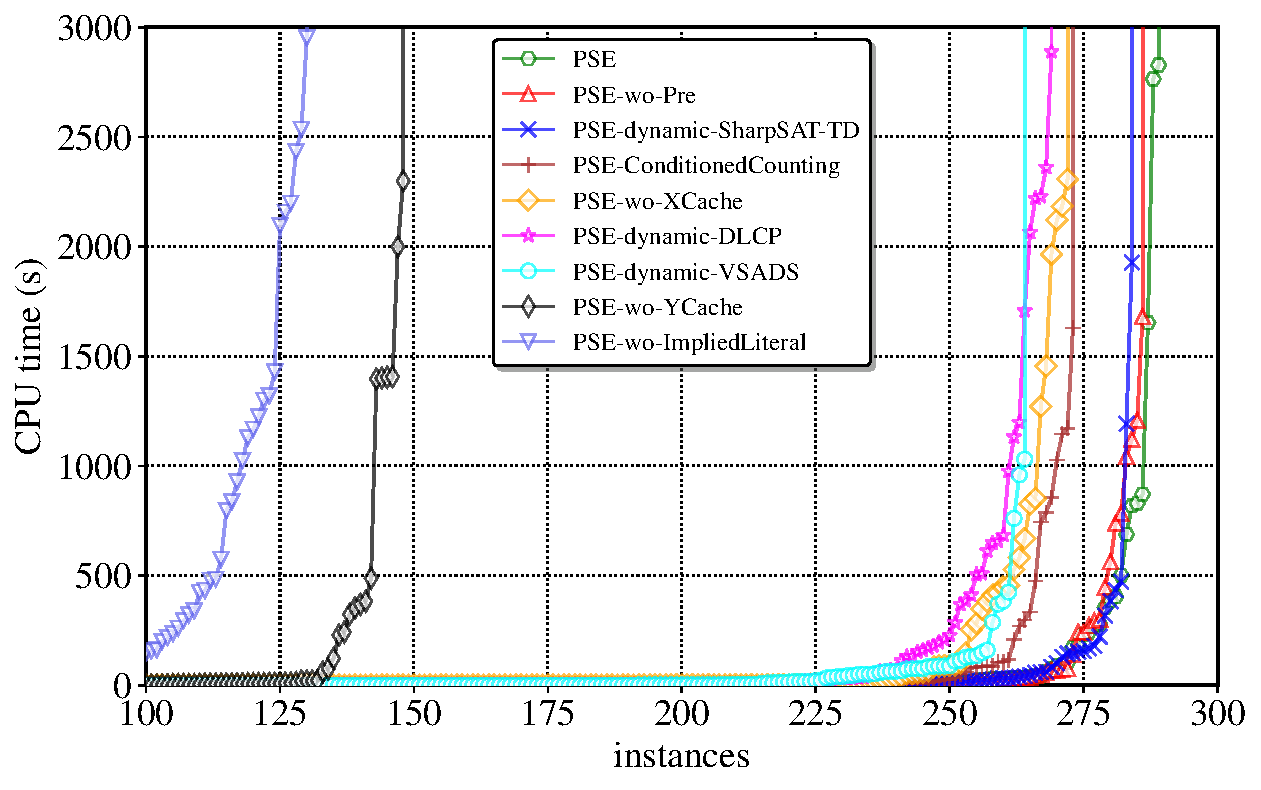
\includegraphics[width=8cm,height=8cm]{figures/Configuration_compare.pdf}
	\caption{Cactus plot comparing different methods.}
	\label{figure:3}
\end{figure} 


\begin{comment}
	\subsection{Impact of pre-process}
	We compare the effects of the preprocessing techniques mentioned in Section 4 on PSE.
	We use the term "Pre" to refer to the preprocessing in ExactMC. "Pre + Liteq" means preprocessing plus literal equivalence strategy. "Pre + Liteq\_New" refers to preprocessing plus the improved literal equivalence strategy proposed in this paper.
	Figure \ref{figure:3} shows the cactus plot comparing three different preprocessing strategies, where the x-axis represents the number of solved instances and the y-axis represents the running time.
	In order to visualise the efficiency gap between different preprocessing methods more intuitively, we removed 250 instances that could be solved by PSE within 1s.
	From the results, it is clear that the literal equivalence strategy is an enhancement to entropy computing and Liteq\_New performs the best. 
	Using literal equivalence strategy can reduce the average PAR-2 score from 1287.38 to 1257.83. while Liteq\_New strategy can make the average PAR-2 score reduced to 1193.37.
	
	
	
	
	\begin{figure}[htbp]
		\centering
		\includegraphics[width=12cm,height=8cm]{figures/Preprocess.pdf}
		\caption{Cactus plot comparing different preprocessing strategies.
		}
		\label{figure:3}
	\end{figure} 
\end{comment}



\section{Related work}
\label{sec:Related}
Our work is based on the close relationship between QIF, model counting, and knowledge compilation.
We introduce relevant work from three perspectives: (1) quantitative information flow analysis, (2) model counting, and (3) knowledge compilation.

\textbf{Quantified information flow analysis} 
Currently, the QIF method based on model counting faces two major challenges. 
The first one is to construct the logical postcondition $\Pi_{proc}$ for a program $proc$~\cite{zhou2018static}.
This process can be achieved through symbolic execution, but the existing symbolic execution tools have certain limitations and are difficult to be extended to some complex programs, such as those involving symbolic pointers.
The second challenge is model counting.
Our work focuses on the challenges of model counting. 
For programs modeled by Boolean clause constraints, Shannon entropy can be solved through model counting queries to quantify the amount of information leakage.
Golia et al. have made outstanding contributions to this work. They proposed the first efficient Shannon entropy estimation\cite{golia2022scalable} with PAC guarantees based on sampling and model counting.
Their core idea is to reduce the number of model counting queries through sampling. However, their idea can only provide an approximate estimation of entropy.
Our work is inspired by the research conducted by Golia et al., but our approach and optimization direction differ. 
We optimize the existing framework of model counting for precise Shannon entropy to reduce the number of model counting queries, while simultaneously enhancing the efficiency of model counting solutions. 
Based on this idea, we propose an efficient and precise method for computing the Shannon entropy.
Besides Boolean clause constraints, converting programs into strings and SMT constraints has also attracted extensive research.
For string constraints, Aydin et al.~\cite{aydin2018parameterized} proposed an automata-based model counting solver, MT-ABC, which can be applied to QIF.
Similar solvers also include SMC~\cite{luu2014model}, ABC~\cite{aydin2015automata}, etc. 
The difference between their methods lies in the improvement of the automaton model counting.
Phan et al.~\cite{phan2014abstract} proposed an abstract model counting method, a quantified information leakage method based on an SMT-based framework.
For approximate estimation of leakage, there are many sampling-based methods. 
The most outstanding work currently is the first efficient Shannon entropy estimation with PAC guarantees proposed by Golia et al.~\cite{golia2022scalable}, which is based on sampling and model counting.

\textbf{Model counting}
Since the computation of entropy relies on model counting, we conducted a survey on powerful techniques for model counting.
%In the model counting problem, the algorithm can be divided into exact model counting and approximate model counting based on the accuracy of the solution.
%In exact model counting, the initial algorithm was based on DPLL search, and researchers gradually proposed some optimization strategies, such as cache and component decomposition.
%Since the 21st century, scalable model counters have been mainly divided into three methods~\cite{lai2021power}: (1) search-based, (2) knowledge compilation-based, and (3) variable elimination-based methods. Among these, model counters based on knowledge compilation have received considerable attention in recent years.
Among the existing techniques for exact model counting, the most effective ones mainly include component decomposition, caching, Implicit Binary Constraint Propagation (i-BCP), variable decision heuristics, preprocess, and so on.
The key idea of the disjoint component analysis is to divide the constraint graph into several parts without variable intersection.
However, this idea is not applicable to the computation of Shannon entropy, as the variables in $Y$ do not support component decomposition.
Caching technique has been used in various fields for a long time, and it also has excellent effects in model counting.
Bacchus et al. analysis three distinct caching schemes: simple caching, component caching,and linear-space caching \cite{bacchus2003dpll}. 
Their research showed that component caching has the most strong prospect. 
Combining component caching with conflict driven clause learning is an idea pioneered by Sang et al \cite{sang2004combining} in 2004 with their model counter Cachet which is based on the well-known SAT solver zCHaff \cite{moskewicz2001chaff}. 
We also utilized caching technique in the process of computing entropy, and our experiments once again demonstrated the power of caching technique.
Thurley \cite{thurley2006sharpsat} proposed improved component encoding schemes with a solver called sharpSAT to make cache components more concise. 
sharpSAT first employed i-BCP in model counting, which is an improvement of the well-known "look-ahead" technique based on Boolean constraint propagation. 
The computation of implied literals relies on IBCP, and our experiments have shown that implied literals are also beneficial to the process of computing entropy.
Sharma et al.~\cite{sharma2019ganak} proposed a probabilistic caching strategy in their model counter Ganak, demonstrating its efficiency.
Our tool PSE does not currently integrate a probabilistic caching method, which is a direction for future exploration. 
There have been many studies on variable decision heuristics for model counting, which can be divided into static heuristics and dynamic heuristics. 
In static heuristics, the \textbf{minfill}~\cite{darwiche2009modeling} heuristic is very effective, while in dynamic heuristics, \textbf{VSADS}~\cite{sang2005heuristics}, \textbf{DLCP}~\cite{lai2021power}, and \textbf{SharpSAT-TD  heuristic}~\cite{korhonen2021integrating} have been the most significant in recent years. 
We have already discussed the impact of these heuristics on entropy computation in Section \ref{sec:Experiments}.
Preprocessing methods in model counting have been discussed in detail by Lagniez et al~\cite{lagniez2017preprocessing}. 
Not all preprocessing methods in model counting are suitable for entropy computation. 
Our research found that the most effective method is literal equivalence, and we have made some improvements to this preprocessing method to make it suitable for entropy computation (in Section \ref{sec:PSE}).

\textbf{Knowledge compilation} %Knowledge compilation compiles propositional theory into a specific target language, which supports querying a variety of queries, including satisfiability, model counting, uniform sampling in polynomial time, etc. 
The motivation for utilizing knowledge compilation for model counting lies in the fact that it is difficult to compute the number of models for the original Boolean formula, whereas the new target language can solve the model counting problem quickly. 
Darwiche et al. first proposed a compiler called c2d~\cite{darwiche2004new} to convert the given CNF formula into Decision-DNNF. 
The core technique of c2d compile CNF to Decision-DNNF is decomposition.
Based on the exact solver sharpsat~\cite{thurley2006sharpsat}, Muise and McIlraith et al. developed a new compiler, Dsharp~\cite{muise2012d}, which converts CNF to Decision-DNNF. 
Unlike c2d, Dsharp utilizes two significant features of sharpSAT: dynamic decomposition and implicit binary constraint propagation. 
Lagniez and Marquis~\cite{lagniez2017improved} proposed an improved Decision-DNNF compiler, called D4, is a top-down compiler that compiles CNF formulas into d-DNNF.
Similar to Dsharp, D4 also uses dynamic decomposition, although the decomposition strategy is different.
In order to better improve the efficiency of the algorithm, D4 makes full use of heuristic strategies such as disjoint component analysis, component caching, conflict analysis and non-technical backtracking, which perform well in c2d and Dsharp. 
Exploiting literal equivalence, Lai et al.~\cite{lai2021power} proposed a generalization of Decision-DNNF, called CCDD, to capture literal equivalence. 
They demonstrate that CCDD supports model counting in linear time and design a model counter called ExactMC based on CCDD.

\begin{comment}
	Later, Darwiche et al. proposed the method of knowledge compilation, which sparked a wave of computing model counting through knowledge compilation, giving birth to many well-known solvers such as c2d~\cite{darwiche2004new}, dsharp~\cite{muise2012d}, d4~\cite{lagniez2017improved}, ExactMC~\cite{lai2021power}, etc.
\end{comment}
%The interaction between logic and probability has garnered significant interest throughout the evolution of AI.
%Within the realm of propositional logic, this interaction has predominantly centered around computational advancements.
%%An important finding is that probabilistic reasoning can be reduced to weighted model counting~\cite{}.

In order to compute the Shannon entropy, the focus of this paper is to design a compiled language that supports the representation of probability distributions.
%Probabilistic inference is a difficult problem in Artificial Intelligence~\cite{dagum1993approximating}.
%Many knowledge compilation languages are used to solve probabilistic problems.
Numerous target representations have been used to concisely model probability distributions, providing more concise factorizations than Bayesian networks in the presence of local structure\cite{dal2021compositional}.
d-DNNF can be used to compile relational Bayesian networks for exact inference~\cite{chavira2006compiling}.
Probabilistic Decision Graph (PDG) is a representation language for probability distributions based on BDD~\cite{jaeger2004probabilistic}.
Probabilistic Sentential Decision Diagram (PSDD) is a complete and canonical representation of probability distributions defined over the models of a given propositional theory~\cite{kisa2014probabilistic}. 
Each parameter of a PSDD can be viewed as the (conditional) probability of making a decision in a corresponding Sentential Decision Diagram (SDD).
And/Or Multi-Valued Decision Diagrams (AOMDDs)~\cite{mateescu2008and} take advantage of the AND/OR structure to represent probability distributions.
Affine ADDs(AADDs)~\cite{sanner2005affine}, an extended form of ADDs, achieve more compression through affine transformations, which is beneficial for probabilistic inference algorithms.
Macii and Poncino~\cite{macii1996exact} demonstrated that ADD enables efficient and precise computation of entropy.
Nevertheless, our experiments revealed that the size of ADD frequently grows exponentially when handling large circuit formulas, suggesting that ADD is not suitable for computing entropy of large-scale circuit formulas.
Based on the core idea of simplifying the size of ADD, we propose an extended form of ADD, ADD-L, which utilizes the power of implied literals to make the graph structure more concise and easier to hit the cache during the construction process.
Apart from ADD, there have been studies utilizing BDDs for approximating entropy.
Stanković et al.~\cite{stankoviccomputing} observed that the process of computing entropy estimates could be implemented on BDDs, thus avoiding redundant calculations and ensuring the efficiency of the process.
They used BDDs to estimate the entropy of a given vector in further studies~\cite{stankovic2007calculating}.
The complexity of their proposed algorithm is proportional to the number of nodes in the decision graph, which is similar to the complexity of our entropy calculation. However, it is worth noting that they only estimated the entropy, while we solve it precisely. 
In addition, the number of ADD-L nodes proposed by us is significantly less than that of BDDs, theoretically making our efficiency much higher.



\begin{comment}
	An efficient approach is trying to find the most concise factorization of the function that computes marginal probabilities, which is also referred to as Knowledge Compilation.
	Numerous target representations have been used to concisely model probability distributions, providing more concise factorizations than Bayesian networks in the presence of local structure\cite{dal2021compositional}.
	Examples include d-DNNF~\cite{chavira2006compiling}, Sentential Decision Diagrams (SDD)~\cite{choi2013compiling}, Probabilistic SDDs (PSDD)~\cite{kisa2014probabilistic}, Reduced Ordered Binary Decision Diagrams (ROBDD)~\cite{nielsen2013using}, Zero-suppressed BDDs (ZBDD)~\cite{minato2007compiling}, And/Or Multi-Valued Decision Diagrams (AOMDDs)~\cite{mateescu2008and}, Probabilistic Decision Graphs (PDG)~\cite{jaeger2004probabilistic}, Weighted Positive BDDs (WPBDD)~\cite{dal2017weighted}, Algebraic Decision Diagrams (ADD)~\cite{dudek2020addmc}, among others.
	
\end{comment}



\begin{comment}
	Many problems in artificial intelligence, after formalization, can be reduced to the problem of calculating the number of models of propositional expressions.
	For example, in the calculation of belief degree and Bayesian belief network in approximate reasoning, approximation can be used to avoid computational difficulties and reduce them to the problem of model counting in the propositional domain~\cite{roth1996hardness}. 
	The probabilistic inference problem can be simplified to the weighted model counting problem on the propositional knowledge base by encoding the Bayesian network into a CNF knowledge base and assigning weights to the CNF variables according to the network probability~\cite{chavira2008probabilistic}. 
	The purpose of assigning weights to variables is to enable each CNF model to generate a weight, which allows people to express the probability of certain evidence as the sum of weights of models consistent with the evidence.
	
	
	In the model counting problem, the algorithm can be divided into exact model counting and approximate model counting based on the accuracy of the solution.
	Exact model counting can accurately solve all the model numbers of the propositional formula, while approximate model counting can only find the model numbers with certain errors or the upper and lower bounds of the real model numbers. 
	Accurate solutions are expected, but at the same time, they take a lot of time to solve, and can only deal with small scale problems, while the approximate model counting sacrifices a certain precision, gets stronger scalability and robustness, and can solve larger scale problems.
	
	
	Therefore, KC-based reasoning techniques are widely used in probabilistic databases~\cite{van2017query}, probabilistic programming~\cite{fierens2015inference}, processable learning~\cite{kisa2014probabilistic}, and synthesis and verification of hardware and software systems~\cite{fried2016bdd}.
	
	Therefore, the compiled formula needs to meet two criteria. Firstly, the size of the formula must be polynomial, otherwise the conversion would be meaningless. Secondly, the speed of computing the model count for the formula must be fast, requiring at least polynomial time complexity, or even linear time complexity.
	In the last two decades, deterministic Decomposable Negation Normal Form (d-DNNF) is a language of wide interest to researchers, supporting the computation of models in polynomial time (within compilation size). 
	In practical applications, binary decision serves as a crucial property that enforces determinism in compiler design~\cite{lagniez2017improved}, and the resulting subset of d-DNNF is referred to as Decision-DNNF~\cite{oztok2014compiling}.
	The state-of-the-art model counter based on knowledge compilation focuses on compilation to a  Decision-DNNF for model counting.
	
	Model counting ($\#$SAT) is the problem of computing the number
	of satisfying assignments for a given propositional formula. It is a fundamental
	problem with a wide variety of applications ranging from
	probabilistic inference~\cite{roth1996hardness, chavira2008probabilistic} , neural network verification~\cite{baluta2019quantitative} , network reliability~\cite{duenas2017counting}, computational biology, and the like. Valiant proved that the problem of model counting is $\#P$ complete~\cite{valiant1979complexity}, where $\#P$ is a set of enumeration problems related to NP decision problems. Later, Todd's pioneering work proved that $PH \subseteq P^{\# P}$  ~\cite{toda1989computational}.
\end{comment}





\section{Conclusion}
\label{sec:Conclusion}

In this paper, we propose a new compilation language, ADD-L, which combines ADD and implied literals to optimize the search process in the first stage of accurate Shannon entropy computation. 
In the second stage of accurate Shannon entropy computation, we optimize model counting queries using shared component cache.
We integrated preprocessing, heuristic, and other methods into the precise Shannon computation tool PSE, with its trace corresponding to ADD-L. 
Experimental results demonstrate that PSE significantly enhances the scalability of precise Shannon entropy computation, even outperforming the state-of-the-art entropy estimator EntropyEstimation in overall performance.
We believe that PSE has opened up new research directions for entropy computing in Boolean formula modeling, such as caching schemes, variable heuristics, preprocessing, etc.
We look forward to designing more suitable techniques for Shannon entropy computation in the future, in order to further enhance the scalability of precise Shannon entropy.


\bibliography{references}
\end{document}

In the $X$-stage, we perform multiple optimized model counting.
PSE, depicted in Algorithm \ref{PSE}, takes in a CNF formula $\varphi$, an input set $X$, and an output set $Y$, and returns the self-information $\mathit{infor}(\sigma, \varphi)$ of the formula, where $\sigma$ is the assignment made in the ancestor calls.
As mentioned in Proposition \ref{prop:Entropy-proposition}, the entropy of the original formula is the output of the root call.


\begin{algorithm}[h]
	\caption{PSE($\varphi$,$X$,$Y$)}
	\label{PSE}
	\LinesNumbered
    \DontPrintSemicolon
	\KwIn{A circuit CNF formula $\varphi$ with inputs $X$ and outputs $Y$}
	\KwOut{the self-information of $\varphi$}
	\lIf{$\varphi = \mathit{false}$} {\Return $0$}
	
	%\If{$\varphi = \mathit{true}$}  { $p \leftarrow 2^{|\varphi| - |Y|}$ \Return $2^{|Y|} \cdot (-p \cdot \log p) $\}
	$n \leftarrow |\mathit{Vars}(\varphi)|$
	
	$L \leftarrow \texttt{GetImpliedLiterals}(\varphi)$ 
	
	$\varphi,Y \leftarrow $\texttt{Simplify}($\varphi, Y, L$) 
	
	\lIf{$\mathit{Cache}(\varphi) \neq nil $} {\Return $\mathit{Cache}(\varphi)$}
	\If{$ Y = \emptyset $}
	{
		$m \leftarrow $ \texttt{CountModels}($\Phi$) 
		
		$p \leftarrow \frac{m}{TotalCount} $
		
		%$\mathit{infor} \leftarrow -p \cdot \log {p}$
		
		\Return  $Cache(\varphi)  \leftarrow 
		-p \cdot \log {p}$
		%\texttt{\mathit{infor}Computing}($\varphi$) $\cdot 2^{|V| - | Vars(\varphi) |}$	
	}
	$ y \leftarrow \texttt{PickGoodVar}(Y)$
	
	$ \varphi_0 \leftarrow \varphi[y \mapsto \mathit{false}]$
	
	$ \varphi_1 \leftarrow  \varphi[y \mapsto \mathit{true}]$
	
	$\mathit{infor}_0 \leftarrow $ PSE($\varphi_0,X,Y \backslash y$)
	
	$\mathit{infor}_1 \leftarrow $  PSE($\varphi_1,X,Y \backslash y$) 
	
	\Return $\mathit{Cache}(\varphi)  \leftarrow $ $2^{n - |\mathit{Vars}(\varphi_0)| - |L| - 1} \cdot  \mathit{infor}_0 +  2^{n - |\mathit{Vars}(\varphi_1)| - |L| - 1} \cdot \mathit{infor}_1$
	%\Return $Cache(\varphi)  \leftarrow \frac{infor_f + infor_t}{2^{|L| + 1}}$
	
\end{algorithm}

We first deal with the cases in which $\varphi$ is $\mathit{false}$ in line 1.  
In such instances where the formula $\varphi$ evaluates to $\mathit{false}$, the self-information associated with the assignment from the ancestor calls is defined as 0.
%When the formula $\varphi$ is $\mathit{true}$, we use a simplification technique where for the remaining unassigned variables $Y$, there are a total of $2^Y$ satisfying assignments.  Therefore, we have $2^{|Y|}$ terminal nodes with a weight of $2^{|\varphi|-|Y|}$ each.
In line 2, we record the number of variables in $\varphi$. 
Subsequently, in line 3, we utilize the \texttt{GetImpliedLiterals} function to extract the implied literals of $\varphi$.
The implementation of \texttt{GetImpliedLiterals} relies on implicit Boolean Constraint Propagation (i-BCP)~\cite{thurley2006sharpsat}. 
In line 4, we simplify both the formula $\varphi$ and the set $Y$ utilizing the extracted implied literals $L$.
Detect whether the simplified formula $\varphi$ has been stored  in the cache in line 5, and return its $\mathit{infor}$ if $\varphi$ hits the cache.
If the current $Y$ is an empty set (in line 6), it means that a satisfiable assignment under the restriction of the output set $Y$ has been obtained. 
We do not explicitly address the case where $\varphi$ evaluates to $\mathit{true}$, as this naturally results in set $Y$ being empty—a defining trait of circuit formulas.
Consequently, the scenario where set $Y$ is empty inherently includes the case where $\varphi$ is $\mathit{true}$.
Lines 7--9 query model counting for the residual formula and calculate its $\mathit{infor}$, corresponding to the terminal case of proposition \ref{prop:Entropy-proposition}.
$TotalCount$ represents the total number of models for the original formula, i.e., for the original formula $\varphi$, $TotalCount= |\mathit{Sol}(\varphi)|$. 
This value is obtained directly through the invocation of any model counter before PSE.
In line 9, the computed self-information $\mathit{infor}$ is cached and then returned as the final result.
If any remaining variables in $Y$ have not been assigned values, we make decisions about them in line 10.
The \texttt{PickGoodVar} function operates as a heuristic algorithm designed to select a variable from set $Y$, with the selection criteria being determined by the specific heuristic employed.
Moving forward, lines 11 and 12 are dedicated to generating the residual formulas $\varphi_0$ and $\varphi_1$, which correspond to the scenarios where the variable $y$ is assigned the values $\mathit{false}$ and $\mathit{true}$, respectively. Following this, lines 13 and 14 are utilized to recursively determine the self-information $\mathit{infor}$ for each of these derived formulas.
Since $\varphi$ is a circuit formula, all residual formulas in the recursive process after the variables in decision $Y$ are also circuit formulas.
Finally, we compute the information for $\varphi$ (corresponding to the non-terminal case of proposition \ref{prop:Entropy-proposition}) and store it in the cache, returning it as the result in line 15.


\subsection{Implementation}

We now discuss the implementation details that are crucial for the runtime efficiency of PSE. 
Specifically, leveraging the tight interplay between entropy computation and model counting, our methodology integrates a variety of state-of-the-art techniques in model counting.

Initially, we have the option to employ various methodologies for the model counting query denoted by \texttt{CountModels} at line 7.
The first considered method is to individually employ state-of-the-art model counters, such as SharpSAT-TD \cite{korhonen2021integrating}, Ganak~\cite{sharma2019ganak}, ExactMC~\cite{lai2021power}, and D4~\cite{lagniez2017improved}.
The second method, called \textbf{ConditionedCounting}, requires the prior construction of a representation of the original formula $\varphi$ to support tractable model counting.
This method is compatible with eligible representation languages such as d-DNNF~\cite{darwiche2004new}, OBDD[$\land$]~\cite{lai2017new}, and SDD~\cite{choi2013compiling}.
Upon reaching line 7, the algorithm executes conditioned model counting, utilizing the compiled representation of the formula and incorporating the partial assignment derived from the ancestor calls.
The last method, called \textbf{SharedCounting}, also solves model counting query by invoking the exact model counter.
Distinct from the first method, \textbf{SharedCounting} does not merely perform model counting in isolation.
Instead, it leverages a shared component cache within the counter across all model counting queries, a strategy we term \textbf{XCache}.
To distinguish it from the cache method in the $X$-stage, we refer to the cache method in the $Y$-stage as \textbf{YCache} in the following.
To differentiate it from the caching approach used in the $X$-stage, the caching method employed in the $Y$-stage is referred to as \textbf{YCache}.
Our observations indicate that the \textbf{SharedCounting} method is most effective within the PSE framework.

\begin{figure}[!htbp]
	
	\centering
	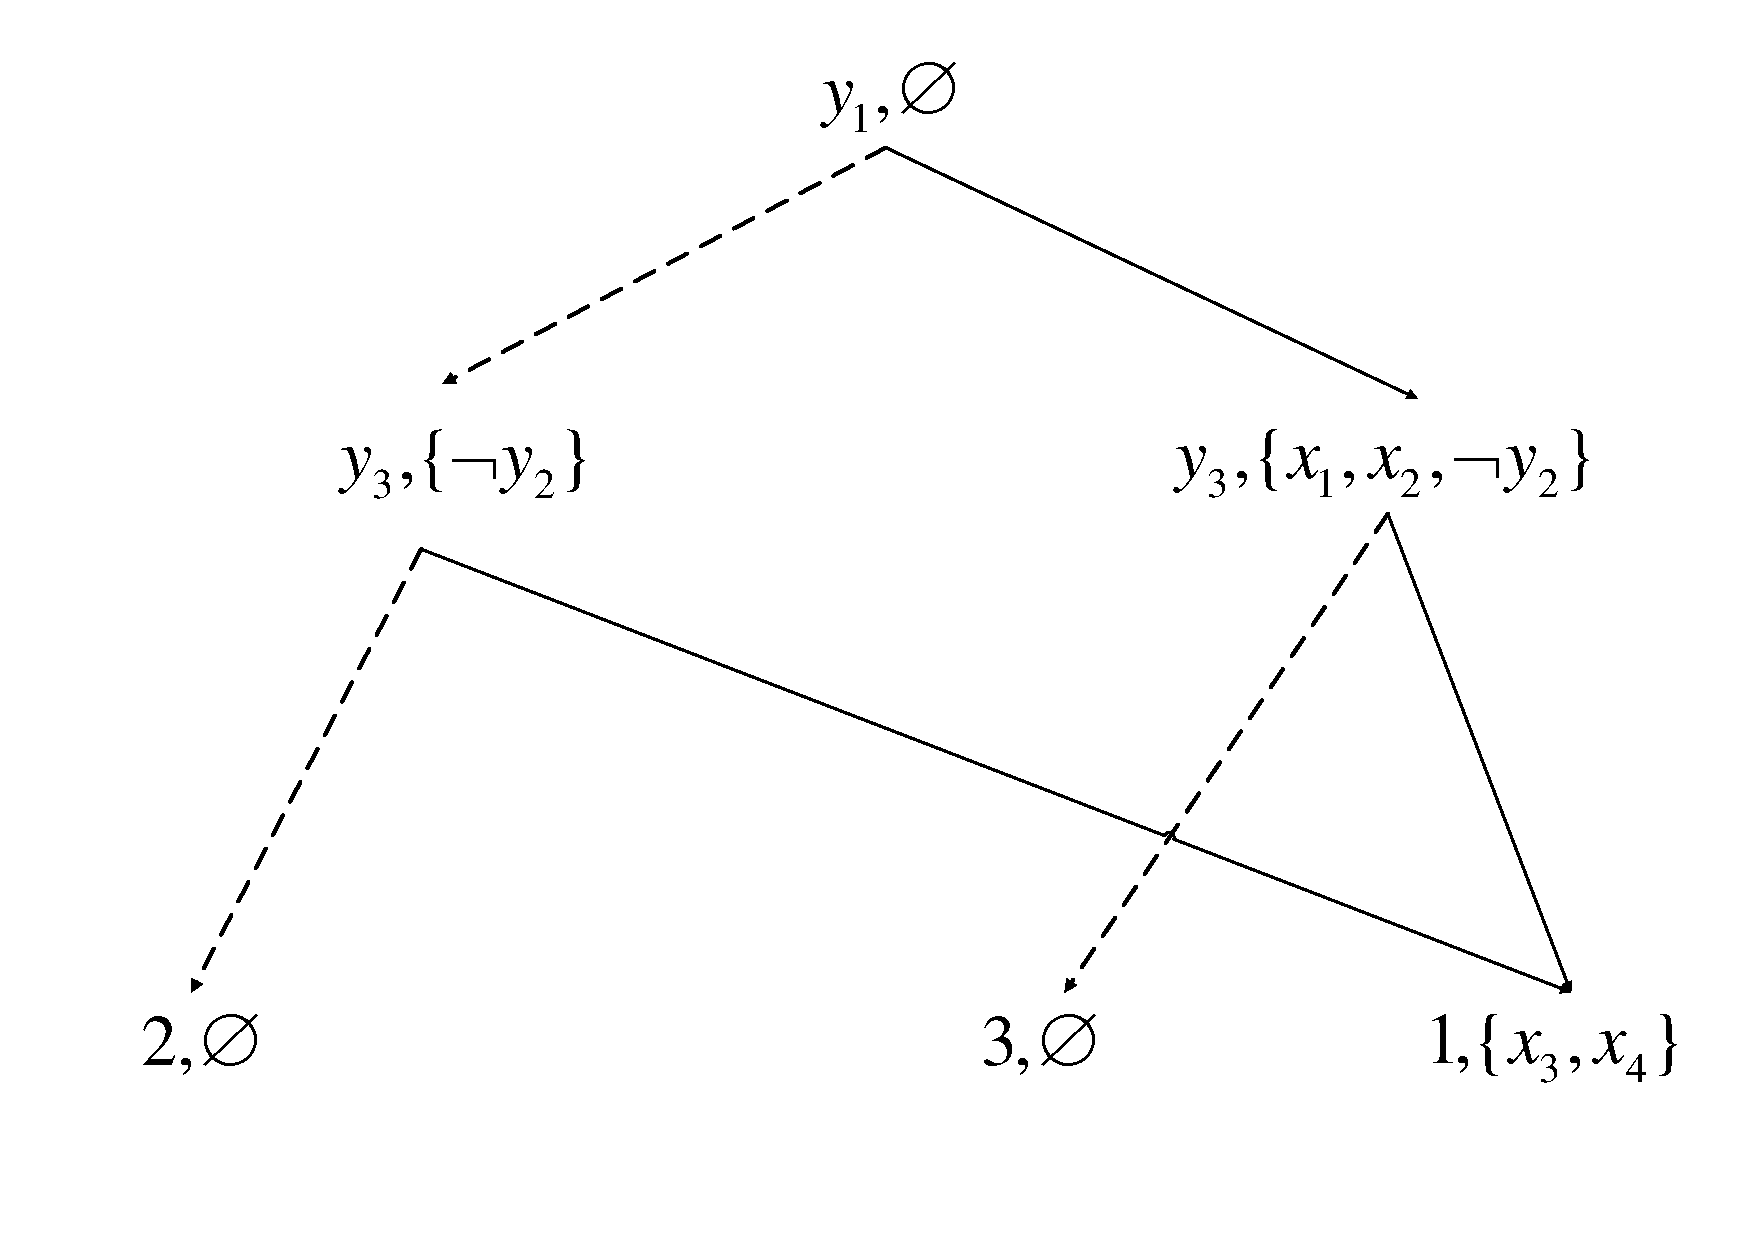
\includegraphics[width=0.7\linewidth]{figures/ADD-L-example2.pdf}
	\caption{An ADD-L example corresponding to Example \ref{circuit-example}, where the implied literals include the variables in $X$. }
	\label{fig:ADDL-example2}
\end{figure} 

\textbf{Implied Literal}
According to the definition of entropy, the assignment $\sigma$ is confined to the variables in set $Y$, implying that, in theory, the implied literals should exclusively involve variables that belong to $Y$.
%However, we observed that if the implied literals are not restricted to only variables in $Y$ and can also include variables in $X$, it can further simplify the formula and optimize the structure of ADD-L.
However, our observations indicate that the ADD-L structure can achieve further simplification and optimization if it is not constrained to implied literals involving only variables in $Y$, but is allowed to encompass variables in $X$ as well.
In light of this insight, we implemented enhancements to the computation of implied literals by lifting the constraints, thus permitting the inclusion of variables from set $X$.
Furthermore, we discovered that employing this technique augments the search efficiency while maintaining the precision of the entropy computation.
To demonstrate the validity and efficacy of this approach, we present an illustrative example in Figure \ref{fig:ADDL-example2}.
%It is easy to see from the comparison between Figure \ref{fig:ADDL-example2} and Figure \ref{fig:ADDL-example1} that this approach optimizes the structure of ADD-L without affecting the entropy result.
From the comparison between Figure \ref{fig:ADDL-example1} and \ref{fig:ADDL-example2}, it is easy to see that the approach optimizes the structure of ADD-L without affecting the entropy result.

\textbf{Variable Decision Heuristic} 
We apply the current state-of-the-art model counting heuristics to the Shannon entropy computing problem and perform experimental comparisons, including \textbf{VSADS}~\cite{sang2005heuristics}, \textbf{minfill}~\cite{darwiche2009modeling}, \textbf{SharpSAT-TD heuristic}~\cite{korhonen2021integrating}, and \textbf{DLCP}~\cite{lai2021power}.
We experimented with these heuristics, and our experiments show that the \textbf{minfill} heuristic is the one that performs best in the entropy computing problem. 
We use the \textbf{minfill} heuristic by default in our subsequent experiments.

\textbf{Preprocessing} 
%Since the core of entropy computing is model counting, we try to integrate the preprocessing strategy in model counting into our entropy tool PSE.
%Based on Literal Equivalences, which is a powerful technique in SAT solving, we implement a new preprocessing approach in PSE.
Since model counting is the core of entropy computing, we extend the preprocessing technique based on literal equivalence in model counting and integrate it into our entropy tool, PSE.
This idea is inspired by the work of Lai et al. \cite{lai2021power} on capturing literal equivalence in knowledge compilation.
However, due to the special nature of the entropy computing process, we cannot arbitrarily replace the literals corresponding to variables in the output set with equivalent ones.
%This is because the new formula $\varphi '$ obtained after the equivalent substitution of literals is equivalent to $\varphi$ in model counting, but not necessarily equivalent in entropy (it is not equivalent when the variables corresponding to the substituted literals belong to $Y$).
%At the beginning, we had a simple idea to restore all equivalent literals after the calculation, in order not to affect the calculation of the entropy and at the same time to reduce the size of the formula.
This is because the new formula $\varphi'$ obtained after the equivalent substitution of literals is equivalent to $\varphi$ in model counting, but not necessarily equivalent in entropy (it is not equivalent when the variables of substituted literals belong to $Y$).
In the beginning, we had the simple idea of restoring all equivalent literals after the calculation so as not to affect the calculation of the entropy and, at the same time, reduce the size of the formula.
We improve this idea by restoring only the literals corresponding to the variables in $Y$, since the assignments that affect the entropy are only in the part of $Y$. 
The new preprocessing method is called \textbf{Pre} in the following.
Experiments have demonstrated that this preprocessing method provides some performance enhancement to the tool (See Section \ref{sec:Experiments}).
This idea of preprocessing is motivated by the fact that, on the one hand, after preprocessing using literal equivalence, it can simplify the formula and thereby improve the efficiency of the subsequent model counting.
On the other hand (and more importantly), it reduces the treewidth of the tree decomposition, which leads to a more optimal order of variable selection obtained by the tree decomposition heuristic, and can be very effective in improving the efficiency of PSE calculations.




\begin{comment}
	Algorithm \ref{Condition} describes another model counting method in $X$-stage.
	To implement this method, a prerequisite is that we need an ADD-L constructed based on the original minfill static variable order. The difference between this ADD-L and the ADD-L corresponding to Algorithm 2 is that the $Y$-stage of Algorithm 2 is equivalent to making decisions only on the variables of the $Y$ set based on the minfill static variable order, while our new idea is to make decisions on all variables in the order of the minfill static variable order (including var in $X$). 
	The motivation for this is that our experiments have found that the heuristic effect of the minfill linear order is much stronger (making decisions only on the variables of the $Y$ set to some extent disrupts the linear order). 
	At this point, the computing process is more like general model counting, which can efficiently construct ADD-L. 
	With such an ADD-L, we can utilize conditional model counting (or entropy computing) in knowledge compilation to solve the model counting in the $X$-stage. 
	Lines 1-2 of the algorithm indicate that when the result of a node hits the cache, we can directly retrieve the corresponding result from the cache. 
	When accessing a terminal node, we directly return the result of the corresponding terminal node (lines 4-5). 
	If the variable decision of node u is false, we recursively call the lo branch to solve it (lines 7-8). 
	Similarly, when the variable decision of node u is true, we recursively call the hi branch to solve it (lines 10-11). Otherwise, it means that the variable corresponding to the node has not been decided, so both lo and hi need to be called (line 13). 
	We cache the current result and return it in lines 14-15.
	
	
	
	If any remaining variables in $Y$ have not been assigned values, we make decisions about them in lines 8-10.
	First, a variable x is chosen heuristically.
	Next the $infor$ of the subformula is computed recursively for two different values (true, false) of $x$. 
	Finally, the $infor$ of the two subformulas ($\varphi[y \mapsto false]$ and $\varphi[y \mapsto true]$) are summed to obtain the $infor$ of the current formula, and the $infor$ associated with the corresponding formula is added to the cache.
	
	Whenever we obtain a satisfiable assignment $\sigma_{\downarrow Y}$ under the restriction of the output set $Y$, we need to calculate the number of different inputs corresponding to this assignment.
	This step can be achieved by performing model counting on the remaining formulas (corresponding to the numerator of $p_{\sigma}$).
	According to \ref{projected-proposition},  the denominator of  $p_{\sigma}$ can be represented by the total number of models of $\varphi$, from which $p_{\sigma}$ can be calculated, and then the $infor$ of the sub-formula can be derived.
	Algorithm \ref{InforComputing} describes this process. 
	
	Algorithm \ref{InforComputing} receives a remaining CNF formula $\Phi$ after all variables in $Y$ have been assigned and returns the $infor$ $H(\varphi)$ of $\Phi$.
	As mentioned above, we perform model counting on the remaining sub-formulas in lines 1-4.
	In the model counting of the $X$-stage, we propose two methods, called \textbf{Counting} and \textbf{Condition}, with $count_{opt}$ as a parameter to indicate the chosen method.
	The first approach corresponds to lines 1-2, where any exact model counting tool can be called. 
	It's worth noting that this method does not just query the model counting individually.
	Instead, we share the component cache for all model counting queries, and we refer to this strategy as \textbf{XCache}.
	The other method requires constructing in advance an ADD-L that contains all the variables in $Y$, which can also include variables from the $X$.
	Then convert the model counting into conditional model~\cite{lai2017new} counting based on the current variable assignment.
	In line 5, probability $p_{\sigma}$ is computed according to the definition in Section 2, where $totalcount$ is the number of models of the entire formula $\varphi$, which is also computed by a model counting tool. 
	We only need to calculate $totalcount$ once and store it. 
	In line 6, the $infor$ can be obtained from $p_{\sigma}$ and returned as a result in line 7.
	
\end{comment}

